\documentclass[12pt,a4paper,titlepage]{book}

\usepackage[utf8]{inputenc}
\usepackage[spanish,es-noquoting]{babel}
\usepackage{amsmath}
\usepackage{amsthm}
\usepackage{amsfonts}
\usepackage{amssymb}
\usepackage{graphicx}
\usepackage{lettrine}
\usepackage{float}
\usepackage{color}
\usepackage[top=3cm,bottom=4cm,outer=2cm,inner=2cm]{geometry}
\usepackage{pgf}
\usepackage{emptypage} 
\usepackage{chngcntr}
\usepackage{etoolbox}
\usepackage{listings}
\usepackage{verbatimbox}
\usepackage{rotating} 
\usepackage{tikz}
\usetikzlibrary{arrows}
\usepackage{tkz-graph}
\usepackage{subfig}
\usepackage[T1]{fontenc}
\usepackage{amsmath}
\usepackage{kbordermatrix}
\usepackage[colorlinks=true,linkcolor=black,urlcolor=black,citecolor=black]{hyperref}

\setlength\parindent{0pt}
\def\labelitemi{$\diamondsuit$}
\usepackage{amsmath}
\usepackage{xparse}
\usepackage{amsthm}
\usepackage{tikz}

% Seno
\def\sen{\mathop{\mbox{\normalfont sen}}\nolimits}

% Seno hiperbólico
\def\senh{\mathop{\mbox{\normalfont senh}}\nolimits}

% Arcoseno
\def\arcsen{\mathop{\mbox{\normalfont arcsen}}\nolimits}

% Gradiente
\def\grad{\mathop{\mbox{\normalfont grad}}\nolimits}

% Argumento principal
\def\Arg{\mathop{\mbox{\normalfont Arg}}\nolimits}

% Logaritmo complejo
\def\Log{\mathop{\mbox{\normalfont Log}}\nolimits}

% Rotacional
\def\rot{\mathop{\mbox{\normalfont rot}}\nolimits}

% Divergencia
\def\diver{\mathop{\mbox{\normalfont div}}\nolimits}

% Longitud
\def\longi{\mathop{\mbox{\normalfont long}}\nolimits}

% Índice de una curva
\def\ind{\mathop{\mbox{\normalfont Ind}}\nolimits}

% Rango de una matriz
\def\rang{\mathop{\mbox{\normalfont rang}}\nolimits}

% Norma
\newcommand{\norm}[1]{\lVert #1 \rVert}

% Derivada parcial
\newcommand{\derpar}[1]{\dfrac{\partial}{\partial #1}}

% Derivada parcial con función
\newcommand{\derparcial}[2]{\dfrac{\partial #1}{\partial #2}}

% Derivada parcial de orden n con funcion
\newcommand{\derparcialn}[3]{\dfrac{\partial^{#3} #1}{\partial #2^{#3}}}

% Integral doble en [a,b] x [c,d]
\newcommand{\intdob}[4]{\displaystyle \int_{#1}^{#2} \int_{#3}^{#4}}

% Integral triple en [a,b] x [c,d] x [e,f]
\newcommand{\inttri}[6]{\displaystyle \int_{#1}^{#2} \int_{#3}^{#4} \int_{#5}^{#6}}

% Números complejos
\def\C{\ensuremath{\mathbb{C}}}

% Números reales
\def\R{\ensuremath{\mathbb{R}}}

% Números racionales
\def\Q{\ensuremath{\mathbb{Q}}}

% Números enteros
\def\Z{\ensuremath{\mathbb{Z}}}

% Números naturales
\def\N{\ensuremath{\mathbb{N}}}

% Teorema
\newtheorem{teo}{Teorema}

% Corolario
\newtheorem{cor}{Corolario}

% Proposición
\newtheorem{prop}{Proposición}

% Lema
\newtheorem{lema}{Lema}

% Definición
\newtheorem{defi}{Definición}

% Observaciones
\newtheorem*{obs}{Observaciones}

\newtheorem*{ob}{Observación}

\newtheorem*{nota}{Nota}

\newtheorem*{problema}{Problema}

\newtheorem*{pregunta}{Pregunta}

\newtheorem{ejemplo}{Ejemplo}

\NewDocumentCommand{\overarrow}{O{=} O{\uparrow} m}{%
  \overset{\makebox[0pt]{\begin{tabular}{@{}c@{}}#3\\[0pt]\ensuremath{#2}\end{tabular}}}{#1}
}
\NewDocumentCommand{\underarrow}{O{=} O{\downarrow} m}{%
  \underset{\makebox[0pt]{\begin{tabular}{@{}c@{}}\ensuremath{#2}\\[0pt]#3\end{tabular}}}{\ensuremath{#1}}
}

\newcommand{\contradiction}{%
\begin{tikzpicture}[rotate=45,x=0.5ex,y=0.5ex]
\draw[color=red, line width=.1ex] (0,2) -- (3,2) (0,1) -- (3,1) (1,3) -- (1,0) (2,3) -- (2,0);
\end{tikzpicture}
}


\newcommand*{\autores}{
	\begin{tabular}{r}
		Javier Jiménez del Peso\\
	\end{tabular}
}

%*******************************************************
%                 NO MODIFICAR
\newcommand*{\FSfont}[1]{%
	\fontencoding{T1}\fontfamily{#1}\selectfont}

\newlength{\tpheight}\setlength{\tpheight}{0.9\textheight}
\newlength{\txtheight}\setlength{\txtheight}{0.9\tpheight}
\newlength{\tpwidth}\setlength{\tpwidth}{0.9\textwidth}
\newlength{\txtwidth}\setlength{\txtwidth}{0.9\tpwidth}
\newlength{\drop}
%*******************************************************

% Crea una portada con los siguientes parámetros
%
% #1 : Título 
% #2 : Subtítulo
% #3 : Autor(es)
% #4 : Tutor(es)
% #5 : Lugar
%

\newcommand*{\portada}[5]{
	\begin{titlepage}
		\begingroup
		%\vspace*{1cm}
		\drop = 0.2\txtheight
		\centering
		\vspace*{0.5cm}
		
\includegraphics[scale=0.8]{./imagenes/logo-urjc}

		\vspace*{1.5cm}
		{\Huge  \textbf{#1}}\\[\baselineskip]
		{\Large{Trabajo Fin de Grado}}\\[\baselineskip]
		
		{\large {Escuela Técnica Superior de Ingeniería Informática}}\\[\baselineskip]
		
		\vspace*{0.5cm}
		
		{\large \textbf{#2}}\\[\baselineskip]
		
		{\large{#3}}\\[\baselineskip]
		
		\vspace*{0.5cm}
		
		{\large \textit{#4}}\\[0.5\drop]
		
		\vspace*{0.5cm}
		
		{Tutores:} \\ 
		{\large \textit{#5}}
		\begin{center}
		\end{center}
		\vfill\null
		\endgroup
	\end{titlepage}
}
%*****************************************************




\begin{document}
	
	\frontmatter
	\portada{Modelos predictivos en rankings}{Trabajo Fin de Grado de Matemáticas}{\autores}{Esther García González \\ Miguel Romance del Río}{Móstoles}
	\tableofcontents
	\listoffigures
	
	
	\mainmatter
	\chapter{Introducción}
Los rankings son algo que forma parte de nuestra vida cotidiana: cuando en el telediario analizan los resultados del CIS (Centro de Investigaciones Sociológicas) en cuanto a la valoración de los líderes políticos, cuando estudiamos el ranking de universidades de España para decidir cuál es la mejor para nuestro futuro, cuando escuchamos en la radio el top 10 de éxitos musicales del momento, cuando antes de echar la Quiniela para la próxima jornada consultamos la posición de cada equipo en la clasificación para decidir por quién apostar que ganará cada partido, incluso cuando hacemos una búsqueda en Google y accedemos al primer enlace que es obtenido a partir del algoritmo PageRank. Estos son solo unos pocos ejemplos de la cantidad de rankings que existen en nuestra sociedad. Y siempre que hablamos de rankings viene asociado el concepto de rating, que es el criterio usado en la ordenación de los elementos del ranking, por ejemplo, los puntos que llevan los distintos equipos en cualquier competición deportiva.\\

El proyecto consiste en crear un módulo de predicción de resultados para la próxima jornada de la Liga BBVA estimando las probabilidades de que gane el equipo local, el visitante o de que empaten en cada partido que se disputará. Este módulo formará parte de una aplicación ya existente que entre otras funcionalidades tiene: obtener estadísticas de las distintas temporadas y equipos de la Liga española de fútbol desde 1928 o el estudio de la competitividad en el fútbol.\\ 

En el capítulo 2 repasaremos todos los conceptos matemáticos relativos a rankings que debemos conocer, ya que serán usados en la aplicación informática.
En él recordaremos la definición matemática de ranking y rating y dos métodos de comparación de rankings que usaremos para calcular la tasa de aciertos de los distintos modelos predictivos en capítulos posteriores.\\ 

En el capítulo 3 plantearemos dos modelos matemáticos para predecir cómo quedará el ranking de la próxima jornada de la Liga. Uno basado en la posición que ocupan los equipos en el ranking y otro basado en su tendencia de los últimos enfrentamientos. Finalmente propondremos uno que consista en combinar ambos. Dentro de cada uno de los modelos existirán distintas alternativas de implementación que propondremos con el objetivo de quedarnos con las que mejor se aproximen al resultado real. 
\newpage
El cuarto capítulo constará de la descripción informática del proyecto. En él comenzaremos presentando la herramienta que ya existe, a la que vamos a incorporar el  módulo de predicción. Posteriormente explicaremos la arquitectura de la aplicación y enumeraremos todas las tecnologías usadas para el proyecto. Finalizaremos mencionando los aspectos más relevantes de la implementación de la aplicación.\\

En el quinto explicaremos el funcionamiento del módulo implementado haciendo uso de la aplicación para realizar la predicción de la próxima jornada.\\

En el último capítulo mostraremos los resultados obtenidos por la aplicación en las últimas temporadas. En él obtendremos distintas estadísticas y compararemos los distintos modelos matemáticos propuestos eligiendo las alternativas de implementación que tengan mayor porcentaje de aciertos.\\


	\chapter{Conceptos previos sobre rankings}
En este capítulo vamos a comenzar explicando los conceptos matemáticos relativos a rankings que serán usados en el resto de la memoria y en el funcionamiento de la aplicación.

\section{Rankings vs Ratings}

\subsection*{Rankings}
\begin{defi} 
	Un \textbf{ranking} de tamaño n es una permutación de enteros desde 1 hasta n, es decir, se trata de una biyección $r: \xi \rightarrow \xi$ donde $\xi = \{1,...,n\}$ es el conjunto de elementos a ordenar.
\end{defi}

Se representan como un vector columna en el que cada posición del vector (que coincidirá con alguno de los elementos que queremos ordenar) se corresponderá con un número entero que indica la posición que ocupa dicho elemento en el ranking.  Si $e$ es un elemento del conjunto a ordenar, $r(e)$ es la posición que ocupa el elemento $e$ en el ranking $r$.\\
 
\begin{ejem} \label{ejem1}
Ejemplo de ranking.
\end{ejem}
\[
\begin{array}{ccc}
\begin{array}{c}
\text{A}\\
\text{B} \\
\text{C} \\
\text{D} \\
\end{array} & \left(\begin{array}{c}
2\\
4\\
1\\
3
\end{array} \right)
\end{array}  
\]
\qed

\subsection*{Ratings}
\begin{defi} 
	Un \textbf{rating} es una lista de puntuaciones numéricas, una por cada elemento, es decir, $\tilde{r}: \xi \rightarrow \mathbb{R}$ donde $\xi = \{1,...,n\}$ es el conjunto de todos los elementos.
\end{defi}

Se representan de forma análoga a los rankings, como un vector columna en el que cada elemento se corresponderá con una puntuación numérica (partidos ganados, perdidos, empatados, puntos a favor,...).

\begin{ejem} \label{ejem2}
Ejemplo de rating.
\end{ejem}
\[
\begin{array}{ccc}
\begin{array}{c}
\text{A}\\
\text{B} \\
\text{C} \\
\text{D} \\
\end{array} & \left(\begin{array}{c}
9\\
3\\
12\\
7
\end{array} \right)
\end{array}  
\]
\qed
\ \\

Ordenando un rating, siempre se obtiene un ranking, pero no a la inversa. Por ejemplo, el ranking del ejemplo \ref{ejem1} es el obtenido a partir del rating del ejemplo \ref{ejem2}.

\section{Comparación de rankings}

\subsection{Tau de Kendall}

\begin{defi} Diremos que un par $(i,j)$ es \textbf{concordante} si la posición relativa entre ambos en las dos listas es la misma, es decir, $i$ aparece por encima de $j$ o $j$ aparece por encima de $i$ en ambos rankings.
\end{defi}

El resultado, que oscila entre -1 y 1, nos da el grado en que un ranking coincide con el otro y lo podemos calcular como se muestra a continuación

\begin{equation}
\tau = \dfrac{n_{c} - n_{d}}{n(n-1)/2}
\end{equation}
donde $n_{c}$ es el número de pares concordantes, $n_{d}$ el de pares discordantes y $n$ número de ítems de los rankings. 

\begin{ejem} Dados los dos rankings que se muestran a continuación vamos a calcular la Tau de Kendall:
\end{ejem}
\begin{center}
\[
\begin{array}{ccc}
\begin{array}{c}
\text{A}\\
\text{B} \\
\text{C} \\
\text{D} \\
\end{array} & \left(\begin{array}{c}
2\\
4\\
1\\
3
\end{array} \right)& \left(\begin{array}{c}
1\\
4\\
2\\
3
\end{array} \right)
\end{array}  
\]
	
$ \tau (r_{1},r_{2}) = \dfrac{5-1}{6}=0.6666667$
\end{center}
\qed

\subsection{Rho de Spearman}
La Rho de Spearman ($\rho$) es la distancia $L_{1}$ entre dos rankings completos $r_{1}$ y $r_{2}$ de tamaño $n$ \cite[Pág 206]{comparacion}. Pero como no es igual de importante la coincidencia de los rankings en las últimas posiciones de la lista como lo es en las primeras vamos a hacerle una pequeña modificación a la definición clásica de la Rho de Spearman (la renombramos como $\phi$) que se muestra en la ecuación (\ref{spearman}). Con esta nueva definición la penalización por las discordancias en los primeros puestos del ranking será mayor que en los puestos bajos de la lista \cite[Pág 207]{comparacion}. 

\begin{equation} \label{spearman}
	\phi = \sum_{i=1}^{n} \dfrac{|r_{1}(i) - r_{2}(i)|}{min\{r_{1}(i),r_{2}(i)\}}
\end{equation}

Cuanto menor es el valor de esta medida, es porque la diferencia de puestos en los rankings entre los equipos  es menor y, por tanto, más similares son los rankings.


\begin{ejem} Dados los dos rankings que se muestran a continuación vamos a calcular la Rho de Spearman:
\end{ejem}
\begin{center}
	\[
	\begin{array}{ccc}
	\begin{array}{c}
	\text{A}\\
	\text{B} \\
	\text{C} \\
	\text{D} \\
	\end{array} & \left(\begin{array}{c}
	2\\
	4\\
	1\\
	3
	\end{array} \right)& \left(\begin{array}{c}
	1\\
	4\\
	2\\
	3
	\end{array} \right)
	\end{array}  
	\]
	
	$ \phi (r_{1},r_{2}) = \frac{|2-1|}{1} + 0 + \frac{|1-2|}{1} + 0 = 2$
	
\end{center}

\qed
	\chapter{Predicción de resultados}

\section{Introducción}
Lo que se pretende hacer en este capítulo es plantear modelos que nos permitan predecir como quedará el ranking al final de la jornada que aún no ha comenzado, para lo que hay que estimar las distintas probabilidades de que gane un equipo, el rival o empaten para cada partido que se va a disputar.\\

Los modelos pueden ser de lo más variados y estar basados en todo tipo de factores y métodos que pueden ser usados para predecir los resultados finales del partido.\\

En \cite{refpred1} podemos encontrar varios modelos que se aplican para predecir los resultados de la liga alemana en las temporadas 1999-2000, 2000-2001 y 2001-2002:\\
Uno basado en los \textbf{mercados de predicción} en el que los precios nos ofrecen una visión agregada de la información pública y privada de la que disponen todos los participantes. El funcionamiento de los mercados de predicción se explica en \cite[Tabla II]{refpred1} y el modelo de cálculo de probabilidades se plantea en \cite[pág 62]{refpred1}.\\
El otro modelo está basado en las \textbf{apuestas} en el que podemos realizar el cálculo de la probabilidades como se plantea en \cite[págs 62, 63]{refpred1} basándonos en las predicciones que realizan los corredores de apuestas para imponer los precios.\\
Son dos métodos de predicción relativamente aceptables teniendo mayor exactitud que otros métodos como el de \textit{selección aleatoria} y el de \textit{victoria del equipo local} con los que se comparan en \cite[págs 64-66]{refpred1}, aunque la tasa de acierto entre los dos modelos propuestos, el de los mercados de predicción y el de las apuestas, son muy similares.\\
Se puede aumentar la exactitud de las predicciones combinando ambos métodos, mediante ponderaciones del 50:50 o aplicando distintas reglas como \textit{solo predecir cuando las previsiones de ambos métodos coincidan} \cite[págs 66-67]{refpred1}.\\

En \cite{refpred2} se aplica el uso de \textbf{redes neuronales} para la predicción. En \cite[Section 2.1.]{refpred2} se explica el diseño de la red BP, cada equipo tendrá tres tipos de redes BP que se corresponden con su fuerza y el problema de clasificación consiste en contrastar las fuerzas de los dos equipos: sí A es más fuerte que B, es concordante o es más débil \cite[Section 2.2.]{refpred2}. Todos los partidos jugados serán los datos usados para el entrenamiento \cite[Section 3.1.]{refpred2} y la capa de salida consta de tres neuronas que se corresponden con la probabilidad de ganar, empatar y perder \cite[Section 3.2.]{refpred2} de forma que se pueda predecir el resultado del enfrentamiento como se muestra en \cite[Section 3.4.]{refpred2}.

En \cite{refpred3} se aplica un modelo autorregresivo integrado de media móvil o ARIMA que se usa en \textbf{series temporales} y que se basa en un conjunto de observaciones que se generan de forma secuencial. En \cite[Section E]{refpred3} se realiza la formulación matemática del modelo y en \cite[Section F]{refpred3} se muestran los resultados y el análisis de aplicarlo a tres equipos (uno de la zona alta, otro de la zona media y otro de la zona baja de la clasificación) de la liga india de críquet en el que se intenta predecir el resultado de los últimos 10 partidos de la temporada.\\

\section{Modelo propuesto}
En la sección anterior hemos visto algunos de los modelos que han sido propuestos para predecir los resultados de un partido que está por disputarse siguiendo distintos criterios, ahora vamos a proceder a plantear uno propio. \\

Para hacer una predicción tenemos que calcular tres probabilidades:
\begin{itemize}
	\item La probabilidad de que $a$ gane a $b$: $P(a-b=1)$.
	\item La probabilidad de que $a$ y $b$ empaten: $P(a-b=X)$.
	\item La probabilidad de que $a$ pierda ante $b$: $P(a-b=2)$.
\end{itemize}
Para estimarlas proponemos tener en cuenta lo siguiente:
\begin{itemize}
	\item La posición relativa en la tabla.
	\item La tendencia de cada equipo a lo largo de los últimos partidos.
\end{itemize}

\subsection*{Probabilidad basada en la posición relativa}
El valor va a depender de $r(a)-r(b)$\footnote{Recordemos que $r(e)$ denota la posición que ocupa el elemento $e$ en el ranking.} cuyo valor pertenece al intervalo $[-(n-1),(n-1)] \backslash \{0\}$ dónde $n$ es el número de equipos que hay en el ranking. En nuestro caso aplicado a la Liga Española de fútbol, dado que participan un total de 20 equipos el intervalo en cuestión es $[-19,19]$.\\
La idea es desarrollar un modelo lineal a trozos y optimizar sus parámetros usando el un histórico de resultados.\\

Lo primero es re-escalar el intervalo $[-19,19]$ en el $[0,1]$ mediante alguna función como por ejemplo
\begin{center}
	$ \psi: [-19,19] \longrightarrow [0,1]$\\
	$ t \longmapsto \dfrac{t+19}{38}$
\end{center}

Ahora debemos definir unos umbrales de victoria para el equipo local, empate y victoria visitante en tres escenarios muy distintos: \textit{el primero contra el último}, \textit{equipos en posiciones consecutivas} y \textit{el último contra el primero}. Gráficamente podemos resumirlo como se muestra en la figura \ref{fig:umbrales}.

\begin{figure}[htb]
		\centering
		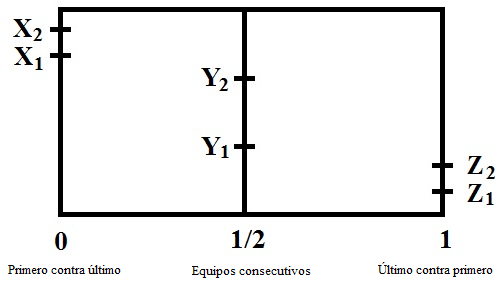
\includegraphics{images/umbrales.png}
		\caption{Gráfico de umbrales de victoria local, empate y victoria visitante.} \label{fig:umbrales}
\end{figure}

Dónde los valores $X_{1},X_{2},Y_{1},Y_{2},Z_{1},Z_{2} \in [0,1]$ se identifican del siguiente modo:
\begin{itemize}
	\item Si $a$ es el primero de la clasificación y $b$ el último:\\
	 $[0,X_{1}]$ mide la probabilidad de que gane $a$, $[X_{1},X_{2}]$ mide la probabilidad de que $a$ y $b$ empaten y $[X_{2},1]$ mide la probabilidad de que gane $b$.
	 Es decir,\\
	 
	 $\begin{cases}
	 	P_{r}(a-b=1)=X_{1}\\
	 	P_{r}(a-b=X)=X_{2}-X_{1} \ \ \ \ \ \ \ \text{siendo} \ 0 \leq X_{1} \leq X_{2} \leq 1\\
	 	P_{r}(a-b=2)=1-X_{2} 
	 \end{cases}$\\
	 
	\item Análogamente, si $a$ y $b$ tienen puestos consecutivos en el ranking:\\
	
	$\begin{cases}
	P_{r}(a-b=1)=Y_{1}\\
	P_{r}(a-b=X)=Y_{2}-Y_{1} \ \ \ \ \ \ \ \text{siendo} \ 0 \leq Y_{1} \leq Y_{2} \leq 1\\
	P_{r}(a-b=2)=1-Y_{2} 
	\end{cases}$\\
	
	\item Finalmente, si $a$ es el último de la clasificación y $b$ el primero:\\
	
	$\begin{cases}
	P_{r}(a-b=1)=Z_{1}\\
	P_{r}(a-b=X)=Z_{2}-Z_{1} \ \ \ \ \ \ \ \text{siendo} \ 0 \leq Z_{1} \leq Z_{2} \leq 1\\
	P_{r}(a-b=2)=1-Z_{2} 
	\end{cases}$
\end{itemize}

Para el resto de escenarios tenemos que interpolar de forma lineal hallando 4 rectas (las que unen $X_{1}$ a $Y_{1}$, $Y_{1}$ a $Z_{1}$, $X_{2}$ a $Y_{2}$ y $Y_{2}$ a $Z_{2}$) tal y como se muestra en la figura \ref{fig:interpolar}.

\begin{figure}[htb]
	\centering
	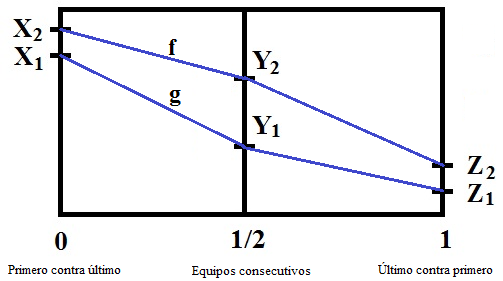
\includegraphics{images/interpolar.png}
	\caption{Gráfica de las funciones resultantes tras realizar la interpolación.} \label{fig:interpolar}
\end{figure}

De esta forma tenemos dos funciones $f,g:[0,1] \longrightarrow [0,1]$ tal que\\
$f(0)= X_{2}$ \ \ \ \ \ $f(1/2)= Y_{2}$ \ \ \ \ \ $f(1)= Z_{2}$ \ \ \ \ \ $f$ recta en $[0,1/2]$ y $[1/2,1]$\\
$g(0)= X_{1}$ \ \ \ \ \ $g(1/2)= Y_{1}$ \ \ \ \ \ $g(1)= Z_{1}$ \ \ \ \ \ $g$ recta en $[0,1/2]$ y $[1/2,1]$\\

De esta forma la predicción queda así\\

$\begin{cases}
	P_{r}(a-b=1)=g(\psi (r(a)-r(b)))\\
	P_{r}(a-b=X)=f(\psi (r(a)-r(b)))-g(\psi (r(a)-r(b)))\\
	P_{r}(a-b=2)=1-f(\psi (r(a)-r(b)))
\end{cases}$
\ \\
\ \\
Para estimar los valores de $X_{1},X_{2},Y_{1},Y_{2},Z_{1},Z_{2}$ hay que optimizarlos teniendo en cuenta las siguientes restricciones:
\begin{itemize}
	\item $X_{1},X_{2},Y_{1},Y_{2},Z_{1},Z_{2} \in [0,1]$
	\item $X_{1} \leq X_{2}$, $Y_{1} \leq Y_{2}$, $Z_{1} \leq Z_{2}$
	\item $X_{1} \geq Y_{1} \geq Z_{1}$ y $X_{2} \geq Y_{2} \geq Z_{2}$	
\end{itemize}

\subsection*{Probabilidad basada en la serie histórica de cada equipo}
Para cada equipo trabajaremos con dos series históricas: una serie con los resultados en casa y otra serie con los resultados fuera de casa, ambos ponderados según una función memoria.\\

Para cada equipo $a$ trabajaremos con secuencias de resultados del tipo:
\begin{center}
	\begin{tabular}{|c|c|c|c|c|c|c|c|c|c|}
	\hline  & t=1 & t=2 & t=3 & t=4 & t=5 & t=6 & t=7 & t=8 & t=9 \\ 
	\hline local (l)  & 1 & 1 & X & 1 & 2 & X & 1 & 1 & 1 \\ 
	\hline visitante (v) & 2 & 2 & X & 2 & 1 & X & 2 & X & 2 \\ 
	\hline 
	\end{tabular} 
\end{center}
De forma que para la jornada siguiente (la t=10) la probabilidad de que el equipo en cuestión gane, empate o pierda como local:
\begin{center}
$P_{l}(a - \star=1)=\dfrac{m(1)+m(2)+m(4)+m(7)+m(8)+m(9)}{\sum_{t=1}^{9}m(t)}$\\
$P_{l}(a - \star=X)=\dfrac{m(3)+m(6)}{\sum_{t=1}^{9}m(t)}$ \ \ \ \
$P_{l}(a - \star=2)=\dfrac{m(5)}{\sum_{t=1}^{9}m(t)}$
\end{center}
donde $m$ es una función memoria típicamente creciente como la de la figura \ref{fig:memoria}.

\begin{figure}[htb]
	\centering
	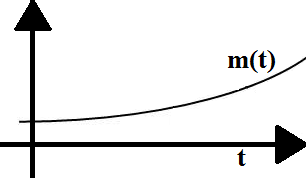
\includegraphics{images/memoria.png}
	\caption{Gráfica de la función memoria.} \label{fig:memoria}
\end{figure}
Análogamente se calculan las probabilidades para el siguiente partido como visitante:
\begin{center}
	$P_{v}(\star - a=1)=\dfrac{m(5)}{\sum_{t=1}^{9}m(t)}$ \ \ \ \
	$P_{v}(\star - a=X)=\dfrac{m(3)+m(6)+m(8)}{\sum_{t=1}^{9}m(t)}$\\
	$P_{v}(\star - a=2)=\dfrac{m(1)+m(2)+m(4)+m(7)+m(9)}{\sum_{t=1}^{9}m(t)}$
\end{center}

Por tanto, para cada equipo tendremos dos probabilidades:\\
$P_{l}(a - \star=1)$, $P_{l}(a - \star=X)$ y $P_{l}(a - \star=2)$ para los partidos como locales \\
$P_{v}(\star - a=1)$, $P_{v}(\star - a=X)$ y $P_{v}(\star - a=2)$ para los partidos como visitantes\\

Para pronosticar el resultado del enfrentamiento $a-b$ debemos conjuntar $P_{l}(a - \star)$ con $P_{v}(\star - b)$ usando la siguiente tabla:\\

\begin{center}
	\begin{tabular}{|c|c|c|c|}
	\hline  & $P_{l}(a - \star=1)$ & $P_{l}(a - \star=X)$ & $P_{l}(a - \star=2)$ \\ 
	\hline $P_{v}(\star - b=1)$ & $(1,0,0)$ & $(\frac{1}{2},\frac{1}{3},\frac{1}{6})$ & $(\frac{1}{4},\frac{1}{2},\frac{1}{4})$  \\ 
	\hline $P_{v}(\star - b=X)$ & $(\frac{1}{2},\frac{1}{3},\frac{1}{6})$ & $(0,1,0)$ & $(\frac{1}{6},\frac{1}{2},\frac{1}{3})$ \\ 
	\hline $P_{v}(\star - b=2)$ & $(\frac{1}{4},\frac{1}{2},\frac{1}{4})$ & $(\frac{1}{6},\frac{1}{2},\frac{1}{3})$ & $(0,0,1)$ \\ 
	\hline 
\end{tabular} 
\end{center}

En las tuplas de números de la tabla anterior, el primer número es el que usaremos para calcular $P_{s}(a-b=1)$, el segundo para $P_{s}(a-b=X)$ y el tercero para $P_{s}(a-b=2)$, dicho número es por el que hay que multiplicar el producto de las entradas.\\
Por ejemplo, para calcular $P_{s}(a-b=1)$ la tabla que debemos usar es la compuesta por el primer elemento de cada tupla\\
\[
A_{1}= \left(\begin{array}{ccc}
1 & 1/2 & 1/4\\
1/2 & 0 & 1/6\\
1/4 & 1/6 & 0
\end{array} \right)
\]
de forma que
	\begin{center}
		$P_{s}(a-b=1)=$
	\end{center}
	$1\cdotp P_{l}(a - \star=1)P_{v}(\star - b=1) + \frac{1}{2}\cdotp P_{l}(a - \star=X)P_{v}(\star - b=1) + \frac{1}{4}\cdotp P_{l}(a - \star=2)P_{v}(\star - b=1)+$\\ 
	$\frac{1}{2}\cdotp P_{l}(a - \star=1)P_{v}(\star - b=X) + 0\cdotp P_{l}(a - \star=X)P_{v}(\star - b=X) + \frac{1}{6}\cdotp P_{l}(a - \star=2)P_{v}(\star - b=X)+$\\
	$\frac{1}{4}\cdotp P_{l}(a - \star=1)P_{v}(\star - b=2) + \frac{1}{6}\cdotp P_{l}(a - \star=X)P_{v}(\star - b=2) + 0\cdotp P_{l}(a - \star=2)P_{v}(\star - b=2)$ \\
\ \\	
Es decir, $P_{s}(a-b=1)= 
\langle
(P_{v}(\star - b=1),P_{v}(\star - b=X),P_{v}(\star - b=2)) A_{1}  
\left(\begin{array}{c}
P_{l}(a - \star=1)\\
P_{l}(a - \star=X)\\
P_{l}(a - \star=2)
\end{array} \right)
\rangle $\\

Aplicaremos un razonamiento análogo para calcular $P_{s}(a-b=X)$ y $P_{s}(a-b=2)$.

\subsection*{Combinación}
Ahora contaremos con dos probabilidades: las probabilidades basadas en la posición relativa ($P_{r}(a-b=1) \ \ P_{r}(a-b=X) \ \ P_{r}(a-b=2)$) y las basadas en la serie histórica de cada equipo ($P_{s}(a-b=1) \ \ P_{s}(a-b=X) \ \ P_{s}(a-b=2)$).\\

Para conjugarlas usaremos una combinación convexa, tomamos $\lambda \in (0,1)$ y tenemos
\begin{center}
	$ P(a-b=1) = \lambda P_{r}(a-b=1) + (1-\lambda) P_{s}(a-b=1)$\\
	$ P(a-b=X) = \lambda P_{r}(a-b=X) + (1-\lambda) P_{s}(a-b=X)$\\
	$ P(a-b=2) = \lambda P_{r}(a-b=2) + (1-\lambda) P_{s}(a-b=2)$
\end{center}
Debiendo optimizar $\lambda$ para obtener el mejor resultado posible entrenándolo sobre el histórico de datos.
	\chapter{Descripción informática}

Vamos a implementar un módulo de predicción de resultados de la Liga BBVA de fútbol en el que aplicaremos los modelos propuestos en el capítulo anterior. Este módulo estará integrado dentro de otra aplicación ya existente que detallaremos a continuación.

\section{Descripción de la aplicación}
\subsection{Arquitectura de la aplicación}
La aplicación está basada en la arquitectura cliente-servidor. Es en la parte del servidor donde se encuentran todas las herramientas relacionadas con la extracción de los datos y la API REST que servirá para interaccionar con la parte del cliente. La parte del cliente constará de la aplicación AngularJS desde donde se realizarán las peticiones a la API REST. En la figura \ref{fig:arquitectura} se muestra la arquitectura de la aplicación.

\begin{figure}[hbt]
	\centering
	\begin{tikzpicture}[database/.style={
		cylinder,
		cylinder uses custom fill,
		cylinder body fill=white,
		cylinder end fill=white,
		shape border rotate=90,
		aspect=0.25,
		draw
	}]
	
	% Base de datos
	\node[database, scale=2] at (5,2.25) (mysql) {MySQL};
	
	% Parser
	\draw (1,1.5) rectangle (3,3.5) node[midway] {PARSER};
	
	% API REST
	\draw (7,1.5) rectangle (9,3.5) node[midway] {API REST};
	
	% APP Angular
	\draw (5,-2.5) rectangle (9,-4.5) node[midway] {Aplicación AngularJS};
	
	% Nube
	\node[cloud, cloud puffs=15, cloud ignores aspect, minimum width=3cm, minimum height=2cm, align=center, draw] (cloud) at (-3, 2.5) {lfp.es};
	
	% Backend
	\draw (0,0) rectangle (10,5);
	
	% Frontend
	\draw (0,-5) rectangle (10,-1);
	
	% Flechas
	
	% Nube - Parser 
	\draw [<-] (1, 2.5) -- node[anchor=south] {HTTP}    (-1.5,2.5);
	
	% Parser - MySQL
	\draw [->] (3, 2.50)   -- node {}  (3.3,2.50);
	
	% API REST - MySQL
	\draw [->] (6.7, 2.25)   -- node {}  (7.00,2.25);
	\draw [<-] (6.7, 2.75)   -- node {}  (7.00,2.75);
	
	% API REST - AngularJS
	\draw [->] (7.5, 1.5)   -- node {}      (7.5,-2.5);
	\draw [<-] (8.5, 1.5)   -- node[anchor=west] {REST}  (8.5,-2.5);
	
	% Backend
	\node at (5,4.75) {\textbf{BACKEND}};
	
	% Frontend
	\node at (5,-1.25) {\textbf{FRONTEND}};
	
	\end{tikzpicture}
	\caption{Arquitectura de la aplicación.} \label{fig:arquitectura}
\end{figure}

\subsection{Funcionalidades previas de la aplicación}
Como ya hemos mencionado, nuestro módulo de predicción forma parte de una aplicación ya existente realizada como parte de otro Trabajo Fin de Grado del que se puede encontrar más información en \cite{tfgjose}. A continuación vamos a mencionar brevemente las funcionalidades de las que constaba antes de añadir el módulo de predicción:

\begin{itemize}
	\item Se pueden consultar los resultados de cualquier temporada de la Primera División de la Liga española de fútbol (desde la 1928/1929 hasta la actual con la excepción del parón sufrido por la Guerra Civil de 1936 a 1939). Por cada temporada se muestra: la clasificación, el histórico de posiciones en el ranking a lo largo de las distintas jornadas, varios gráficos con distintas medidas de competitividad (todas explicadas en \cite[Capítulo 2]{tfgjose}) y el grafo de competitividad.
	\item Se pueden consultar todos los equipos que han jugado al menos en una ocasión en la Primera División de la Liga. De cada uno de ellos se puede consultar su escudo, el número de temporadas que estuvieron en la Primera División y diversas estadísticas sacadas de todos sus partidos disputados.
	\item Se puede iniciar sesión en la aplicación y acceder a un módulo en el que el usuario puede subir como un archivo CSV con un formato concreto (que se puede consultar en \cite[pág 27]{tfgjose}) una secuencia de rankings con el objetivo de crear el grafo de competitividad correspondiente y obtener diversas medidas de competitividad.
\end{itemize}

\section{Herramientas empleadas}
En el desarrollo web se emplea un conjunto muy amplio de tecnologías que se conectan entre sí, podemos crear una aplicación sencilla simplemente usando PHP y MySQL en el lado del servidor y HTML, CSS y JavaScript en el lado del cliente. Además, suelen aparecer otras herramientas asociadas a las anteriores que facilitan la creación de las aplicaciones web, como por ejemplo los frameworks.\\

Partiendo de esto, vamos a proceder a presentar todas las tecnologías usadas en el proyecto, que vamos a separar según las usemos en el lado del cliente o en el lado del servidor.

\newpage

\subsection{Herramientas en el lado del servidor}
El sistema de infraestructura usado en el lado del servidor será la conocida como LAMP, acrónimo de:

\begin{itemize}
	\item \textbf{L}inux, el sistema operativo;
	\item \textbf{A}pache, el servidor web;
	\item \textbf{M}ySQL, el gestor de bases de datos;
	\item \textbf{P}erl, \textbf{P}HP o \textbf{P}ython, los lenguajes de programación (PHP en nuestro caso).
\end{itemize}
\ \\

\subsubsection*{Apache}
\begin{figure}[H]
	\centering
	
\includegraphics{images/apache.png}
	\caption{Apache HTTP Server.}
\end{figure}
El \textit{servidor HTTP Apache} es el servidor web HTTP más usado del mundo, es de código abierto y está disponible para plataformas Windows y Unix entre otras. El servidor Apache es desarrollado y mantenido por una comunidad de usuarios bajo la supervisión de la Apache Software Foundation dentro del proyecto HTTP Server.\\

A parte de ser de código abierto y multiplataforma como ya hemos mencionado, otras de sus principales ventajas son su modularidad y que al ser el más usado es fácil encontrar ayuda y soporte.\\

Para más información se puede acceder a su web desde el siguiente link:\\ \url{http://httpd.apache.org/}

\newpage

\subsubsection*{MySQL}
\begin{figure}[H]
	\centering
	
\includegraphics[scale=0.37]{images/mysql.png}
	\caption{MySQL.}
\end{figure}
\textit{MySQL} es el sistema de gestión de bases de datos relacional más usado del mundo. Sus principales características son que es multiplataforma, multihilo y multiusuario, tiene distintas licencias de uso dependiendo de la finalidad y hace uso de la mayor parte del lenguaje de SQL.\\

Para más información se puede acceder a su web desde el siguiente link:\\ \url{http://www.mysql.com/}

\subsubsection*{PHP}
\begin{figure}[H]
	\centering
	
\includegraphics[scale=0.1]{images/php.png}
	\caption{PHP.}
\end{figure}
\textit{PHP} es un lenguaje de programación de uso general de código del lado del servidor originalmente diseñado para el desarrollo web de contenido dinámico. Fue uno de los primeros lenguajes que se podían incorporar directamente en el documento HTML. Se considera uno de los lenguajes más flexibles, potentes y de alto rendimiento conocidos hasta el día de hoy.\\

Entre sus ventajas destacan que es multiplataforma, libre, fácil de aprender con amplia documentación, tiene tipado dinámico, permite trabajar con gran cantidad de motores de bases de datos, etc.\\  

Para más información se puede acceder a su web desde el siguiente link:\\ \url{http://php.net/}

\subsubsection*{Composer}
\begin{figure}[H]
	\centering
	
\includegraphics[scale=0.55]{images/composer.png}
	\caption{Composer.}
\end{figure}
\textit{Composer} es un gestor de dependencias en proyectos para programación en PHP. Nos permite gestionar (declarar, descargar y mantener actualizados) los paquetes de software en los que se basa nuestro proyecto PHP. \\  

Para más información se puede acceder a su web desde el siguiente link:\\ \url{https://getcomposer.org/}

\subsubsection*{Slim}
\begin{figure}[H]
	\centering
	
\includegraphics[scale=0.1]{images/slim.png}
	\caption{Slim.}
\end{figure}
\textit{Slim Framework} es un micro framework de PHP, sencillo de configurar y que nos permite empezar a programar rápidamente para trabajar con APIs REST de una forma sencilla. \\  

Para más información se puede acceder a su web desde el siguiente link:\\ \url{http://www.slimframework.com/}

\subsubsection*{Java}
\begin{figure}[H]
	\centering
	
\includegraphics[scale=0.85]{images/java.jpg}
	\caption{Java.}
\end{figure}
\textit{Java} es un lenguaje de programación de propósito general, multiplataforma, concurrente y orientado a objetos. Las aplicaciones de Java son generalmente compiladas a bytecode (clase Java) que puede ejecutarse en cualquier máquina virtual Java (JVM) sin importar la arquitectura de la computadora subyacente. \\  

Para más información se puede acceder a su web desde el siguiente link:\\ \url{https://www.java.com/}

\subsection{Herramientas en el lado del cliente}
En esta parte se encuentran todas las tecnologías que definirán la interfaz de interacción con el usuario: el HTML que maqueta la estructura del contenido, el CSS que codifica el diseño y JavaScript que agrega la interacción con el usuario. 
 
\subsubsection*{HTML}
\begin{figure}[H]
	\centering
	
\includegraphics[scale=0.25]{images/html.png}
	\caption{HTML.}
\end{figure}

\textit{HyperText Markup Language} o \textit{HMTL} es el lenguaje de marcado (estándar elaborado por la W3C\footnote{World Wide Web Consortium. Es un consorcio internacional que produce recomendaciones y estándares que aseguran el crecimiento de la World Wide Web.}) usado para la elaboración de páginas web. Define una estructura básica y un código para la definición de contenido de una página web, como texto, tablas, formularios, imágenes o vídeos. Actualmente se encuentra en su versión 5.\\  

Para más información se puede acceder a su web desde el siguiente link:\\ \url{http://www.w3.org/TR/html5/}

\subsubsection*{CSS}
\begin{figure}[H]
	\centering
	
\includegraphics[scale=0.5]{images/css.png}
	\caption{CSS.}
\end{figure}
\textit{Hoja de estilo en cascada} o \textit{CSS} es un lenguaje usado para definir y crear la presentación de un documento estructurado escrito en HTML. La especificación de CSS es también elaborada por la W3C. La idea es separar la estructura de un documento (dada en el HTML) de su presentación (definida por el CSS). En el momento de realización de este documento se encuentra en su versión 3.\\  

Para más información se puede acceder a su web desde el siguiente link:\\ \url{http://www.w3.org/TR/CSS/}

\subsubsection*{JavaScript}
\begin{figure}[H]
	\centering
	
\includegraphics[scale=0.6]{images/js.png}
	\caption{JavaScript.}
\end{figure}
\textit{JavaScript} o \textit{JS} es un lenguaje de programación interpretado, orientado a objetos, imperativo, débilmente tipado y dinámico. Se utiliza principalmente en el lado del cliente, implementado como parte de un navegador web aunque existe una forma de JavaScript del lado del servidor.\\  

Para más información se puede acceder a su web desde el siguiente link:\\ \url{http://www.ecma-international.org/publications/standards/Ecma-262.htm}

\subsubsection*{Bootstrap}
\begin{figure}[H]
	\centering
	
\includegraphics[scale=0.15]{images/bootstrap.png}
	\caption{Bootstrap.}
\end{figure}
\textit{Bootstrap} es uno de los frameworks más populares para trabajar con HTML, CSS y JS en el diseño de sitios y aplicaciones web. La idea es realizar el diseño de una web de forma sencilla mediante el uso de componentes predefinidos.\\

Para más información se puede acceder a su web desde el siguiente link:\\ \url{http://getbootstrap.com/}

\subsubsection*{Bower}
\begin{figure}[H]
	\centering
	
\includegraphics[scale=0.13]{images/bower.png}
	\caption{Bower.}
\end{figure}
\textit{Bower} es un gestor de paquetes JavaScript que se encarga de manejar las
dependencias de paquetes y librerías en el frontend. Bower depende de npm, de Node.js y de git, que debemos de tener previamente instalados.\\  

Para más información se puede acceder a su web desde el siguiente link:\\ \url{http://bower.io/}

\subsubsection*{AngularJS}
\begin{figure}[H]
	\centering
	
\includegraphics{images/angularjs.png}
	\caption{AngularJS.}
\end{figure}
\textit{AngularJS} es un framework de JavaScript para el desarrollo web del frontend que permite crear aplicaciones SPA.\\

Una SPA o Single-Page Application es una aplicación o sitio web que cabe en una sola página con el propósito de simular una aplicación de escritorio. En un SPA todos los códigos de HTML, CSS y JS se cargan de una vez, los recursos necesarios se van cargando dinámicamente cuando lo requiera la página y se van agregando como respuesta de las acciones del usuario.\\  

Para más información se puede acceder a su web desde el siguiente link:\\ \url{https://angularjs.org/}

\section{Implementación}

\subsection{Backend}
El Backend de nuestra aplicación va a constar de dos partes, el parser que obtiene los datos y los almacena en una base de datos de MySQL y la API REST que será la encargada de interaccionar con el frontend haciendo peticiones a la base de datos.\\


\subsubsection{Parser}
El parser es un módulo que consta de varios scripts implementados en PHP cuya función es conectarse a la página oficial de la Liga BBVA de fútbol para descargar los datos jornada a jornada.\\

Consta de:
\begin{itemize}
	\item Un par de scripts que descargan y almacenan en la base de datos el histórico de datos desde la temporada 1928/1929: 
	\begin{itemize}
		\item uno de ellos se encarga de descargar y almacenar las clasificaciones con la posición, el número de puntos, los partidos ganados, empatados y perdidos, los goles a favor y en contra y la diferencia de goles por equipo en cada jornada de la temporada en cuestión,
		\item el otro se encarga de la descarga y almacenamiento de los resultados de cada partido disputado en cada jornada durante la temporada en cuestión. 
	\end{itemize}
	Estos scripts solo deben ejecutarse una vez para almacenar todos los datos pasados.
	\item Un script que se encarga de descargar los resultados de los enfrentamientos de la última jornada y almacenarlos en la base de datos de partidos. Después usando los resultados de esos partidos se calcula el nuevo ranking y se almacena en la base de datos de clasificaciones.\\
	Debemos ejecutar este script cada vez que finalice una jornada, es el que irá actualizando la base de datos en tiempo real.
	\item Un script que se encarga de obtener todos los equipos distintos que aparecen a lo largo de todas las temporadas que tenemos en la base de datos de rankings y los almacena en una base de datos de equipos.
\end{itemize}

\newpage

Los datos obtenidos por los scripts anteriores se irán almacenando en tres bases de datos MySQL distintas cuya estructura se muestra a continuación: 

\begin{itemize}
	\item Tabla de Equipos.
	\begin{figure}[H]
		\centering
		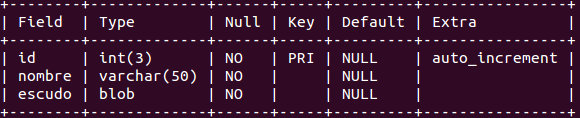
\includegraphics{images/tabla_equipos.png}
		\caption{Estructura de la tabla de equipos MySQL.}
	\end{figure}
	\item Tabla de rankings.
	\begin{figure}[H]
		\centering
		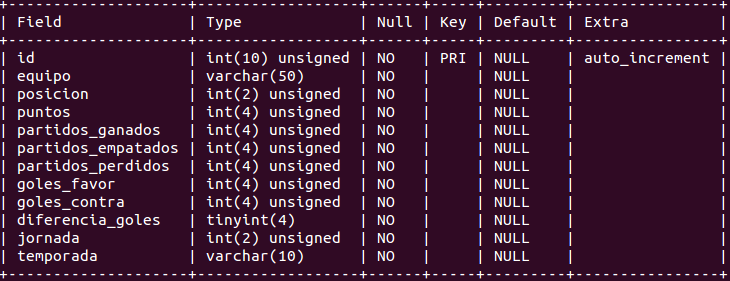
\includegraphics[scale=0.8]{images/tabla_rankings.png}
		\caption{Estructura de la tabla de rankings MySQL.}
	\end{figure}	
	\item Tabla de partidos.
	\begin{figure}[H]
		\centering
		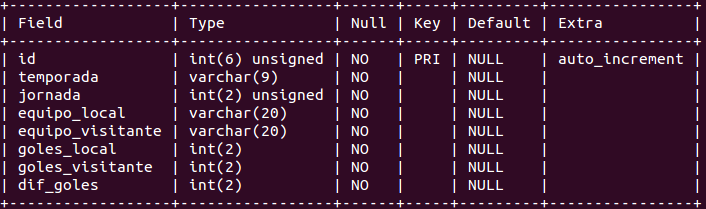
\includegraphics[scale=0.88]{images/tabla_partidos.png}
		\caption{Estructura de la tabla de partidos MySQL.}
	\end{figure}
\end{itemize}

\subsubsection{API REST}
REST (\textbf{RE}presentational \textbf{S}tate \textbf{T}ransfer) es un tipo de arquitectura de desarrollo web definida en el año 2000 por Roy Fielding que se apoya en el estándar HTTP. \\

Existen tres niveles de calidad a la hora de aplicar REST en el desarrollo de una API, que se recogen en el Modelo de Madurez de Richardson\cite{refapi1}\cite{refapi2}:
\begin{itemize}
	\item Nivel 0: consiste en el uso de HTTP como sistema de transporte sin usar otros mecanismos que permite la web.
	\item Nivel 1: vamos a trabajar con información que querremos consultar, modificar o borrar independientemente de su formato, es a lo que denominaremos ``recurso''. Estos recursos deben de tener una URL (Uniform Resource Locator) única que lo identifique y nos permita acceder a su ubicación.
	\item Nivel 2: consiste en la incorporación de los métodos HTTP (GET para consultar, POST para crear, PUT y PATCH para editar y DELETE para eliminar) así como los distintos códigos de estado que devuelve HTTP.
	\item Nivel 3: HATEOAS (Hypertext As The Engine Of Application State) consiste en conectar mediante hipervínculos las aplicaciones clientes con las APIs, permitiendo a dichos clientes despreocuparse por conocer de antemano del cómo acceder a los recursos.
\end{itemize}

\begin{figure}[H]
	\centering
	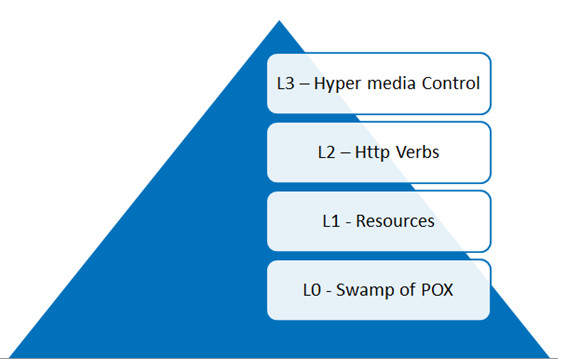
\includegraphics{images/apirest.png}
	\caption{Modelo de Madurez de Richardson.}
\end{figure}

La API implementada llega hasta el nivel 2 del Modelo de Madurez de Richardson. La herramienta que hemos empleado en su implementación es PHP con ayuda del micro framework Slim, que es de gran utilidad para la creación de APIs.\\

En \cite[Anexo A]{tfgjose} se pueden encontrar todos los métodos de la API REST que se encontraban previamente implementados en la aplicación. Para el intercambio de información entre cliente y servidor usaremos el formato JSON por su simplicidad. \\

Al incluir el nuevo módulo de predicción hemos tenido que incorporar una nueva llamada a la API:
{\small \begin{center}
	\begin{tabular}{|c|c|}
	\hline URL  & /sport/:sportname/:league/prediction \\ 
	\hline Método & GET \\ 
	\hline Descripción & Devuelve la predicción para la próxima jornada de la liga :league del deporte :sportname\\ 
	\hline 
\end{tabular} 
\end{center}}

La llamada anterior devuelve un JSON que consta de 6 elementos, en orden:
\begin{enumerate}
	\item las probabilidades de resultados de los partidos calculadas por el modelo de interpolación,
	\item el ranking resultante usando el modelo de interpolación,
	\item las probabilidades de resultados de los partidos calculadas por el modelo de tendencias,
	\item el ranking resultante usando el modelo de tendencias,
	\item las probabilidades de resultados de los partidos calculadas por la combinación de los dos modelos, y
	\item el ranking resultante usando la combinación de los dos modelos.
\end{enumerate}

\begin{figure}[H]
	\centering
		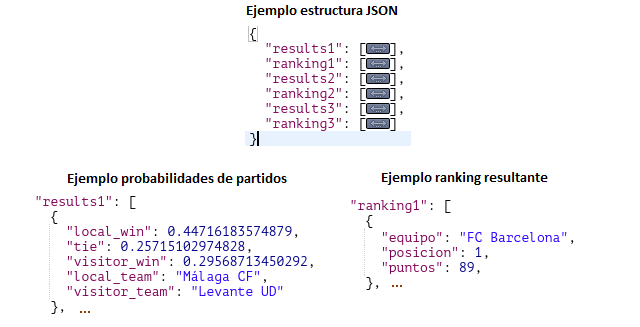
\includegraphics[scale=0.8]{images/json.png}
	\caption{Ejemplo del JSON devuelto por la API.}
\end{figure} 
\ \\
Para obtenerlos se hace uso de funciones implementadas en distintos scripts PHP que realizan los cálculos matemáticos explicados en el capítulo 3 de esta memoria. \\

Para realizar la predicción aplicando el modelo de interpolación necesitamos obtener los umbrales que vamos a usar en los cálculos de las probabilidades. Para ello usaremos una clase Java que obtiene los umbrales desde la temporada que pongamos como inicio hasta la actual y los exporta como un archivo de texto.\\

Para realizar la predicción aplicando la combinación convexa de los dos modelos necesitamos ``entrenar'' sobre un histórico de datos y quedarnos con el valor de $\lambda$ que mejores resultados obtenga. Para ello usamos un script que prueba todos los valores de $\lambda$ desde $\lambda=0$ hasta $\lambda=1$ aumentando en cada paso $0.01$. Una vez obtenido el valor óptimo de $\lambda$ lo fijamos en el script que calcula las probabilidades.  

\subsection{Frontend}
El frontend consta de la aplicación AngularJS que será la encargada de hacer peticiones a la API REST y mostrar los resultados devueltos.\\

Tendremos que crear las vistas y controladores correspondientes al nuevo módulo de predicción añadido. En el controller se realizará la petición a la API REST y se guardará la respuesta obtenida en el contexto para su posterior uso en el HTML correspondiente. También tendremos que modificar todas las demás vistas y controladores para poder acceder al nuevo módulo desde el resto de vistas ya existentes.\\

Todos los aspectos relacionados con las vistas con las que ya contaba la aplicación anteriormente se pueden encontrar en \cite[sección 3.4.1.]{tfgjose}.\\


\subsubsection{Vista del módulo de predicción}
En la figura \ref{fig:pprinc} se muestra la vista principal de la aplicación cada vez que la iniciamos. En la esquina superior derecha aparece el formulario desde el que podemos registrarnos o iniciar sesión para acceder al módulo de subir nuestros propios rankings. En el lateral izquierdo aparecerán todas las temporadas desde 1928/1929 hasta la más reciente, todos los equipos que han jugado alguna vez en Primera División y nuestro recién añadido módulo de predicción de resultados deportivos.\\

Cuando accedamos al módulo de predicción nos aparecerá una vista que consta de tres partes, cada una de ellas con dos tablas (las probabilidades de los resultados de los partidos de la próxima jornada y la predicción de la clasificación), que se corresponden respectivamente con cada uno de los tres modelos propuestos, el basado en la posición de los equipos (figura \ref{fig:pmod1}), el basado en la tendencia de los equipos en los últimos partidos (figura \ref{fig:pmod2}) y la combinación de ambos (figura \ref{fig:pmod3}).

\newpage

\begin{figure}[H]
	\centering
	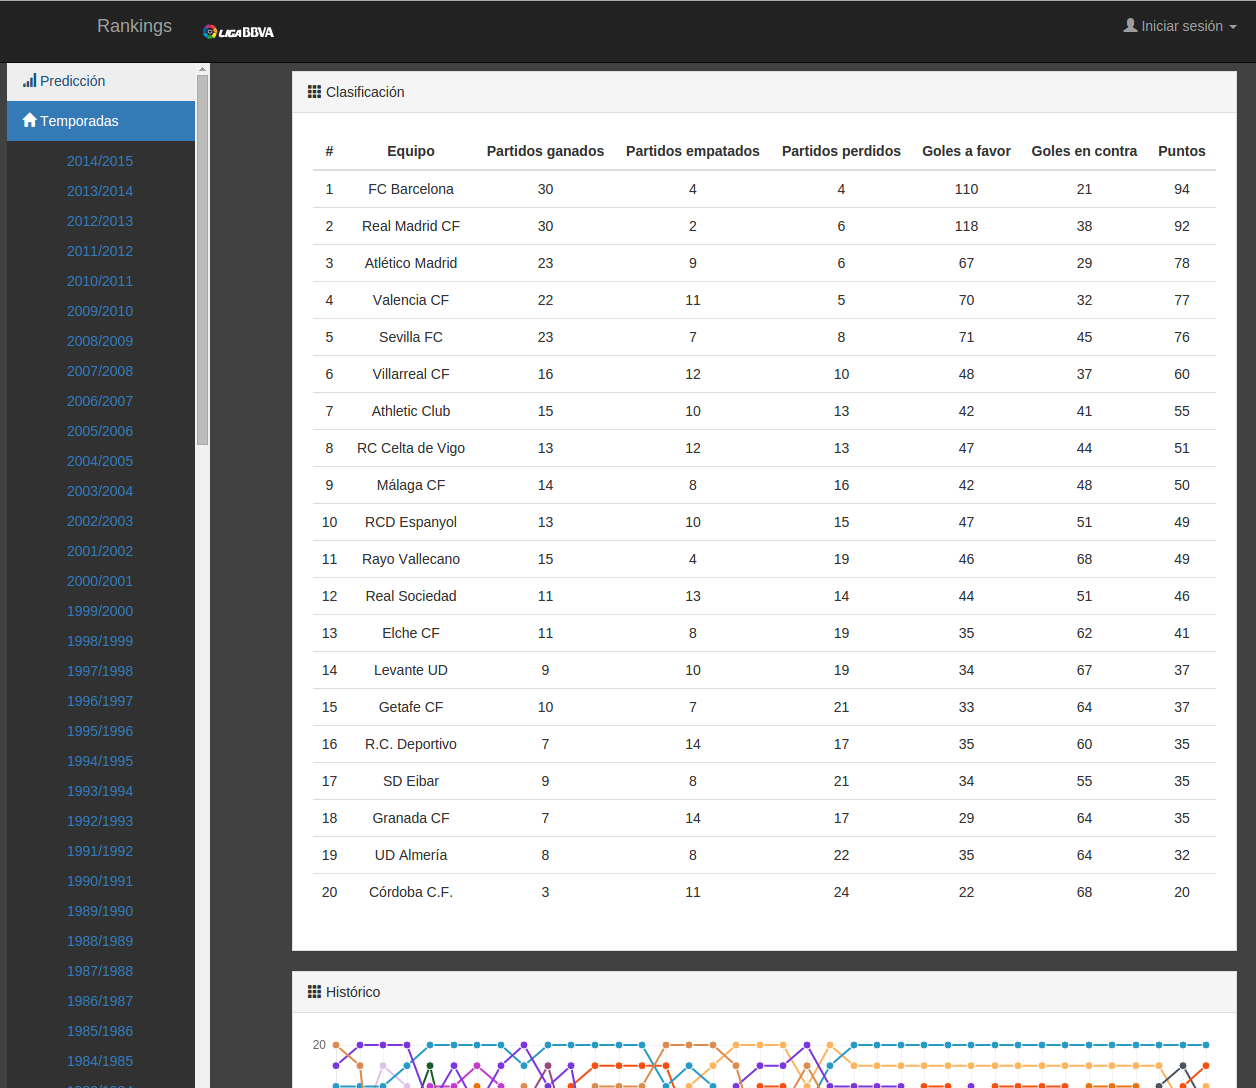
\includegraphics[scale=0.525]{images/pant_principal.png}
	\caption{Pantalla principal de la aplicación.} \label{fig:pprinc}
\end{figure}
\begin{figure}[H]
	\centering
	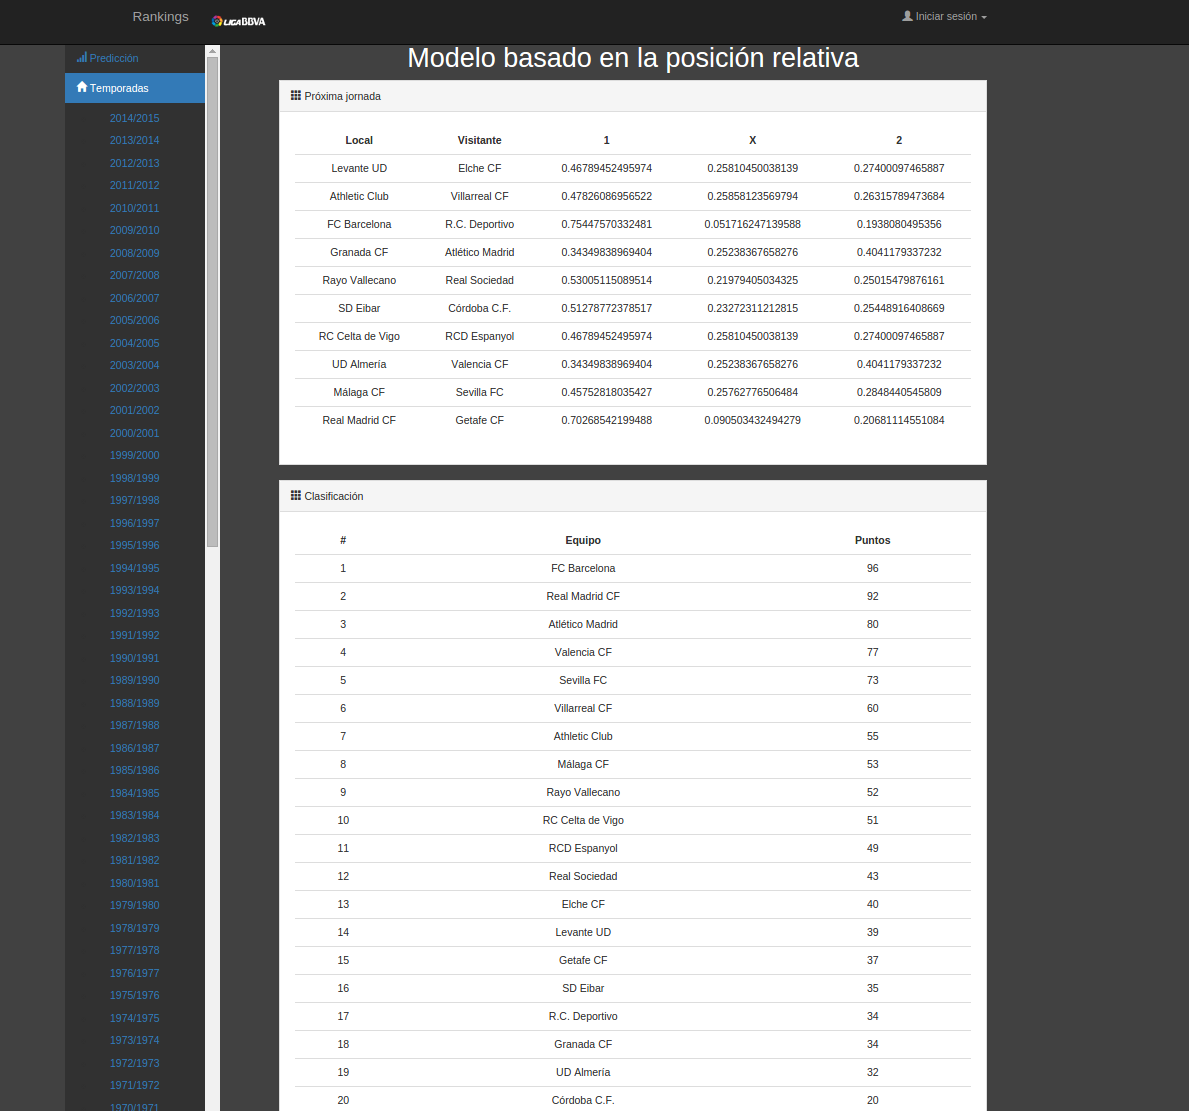
\includegraphics[scale=0.55]{images/pant_pred1.png}
	\caption{Vista del modulo de predicción(I).} \label{fig:pmod1}
\end{figure}
\begin{figure}[H]
	\centering
	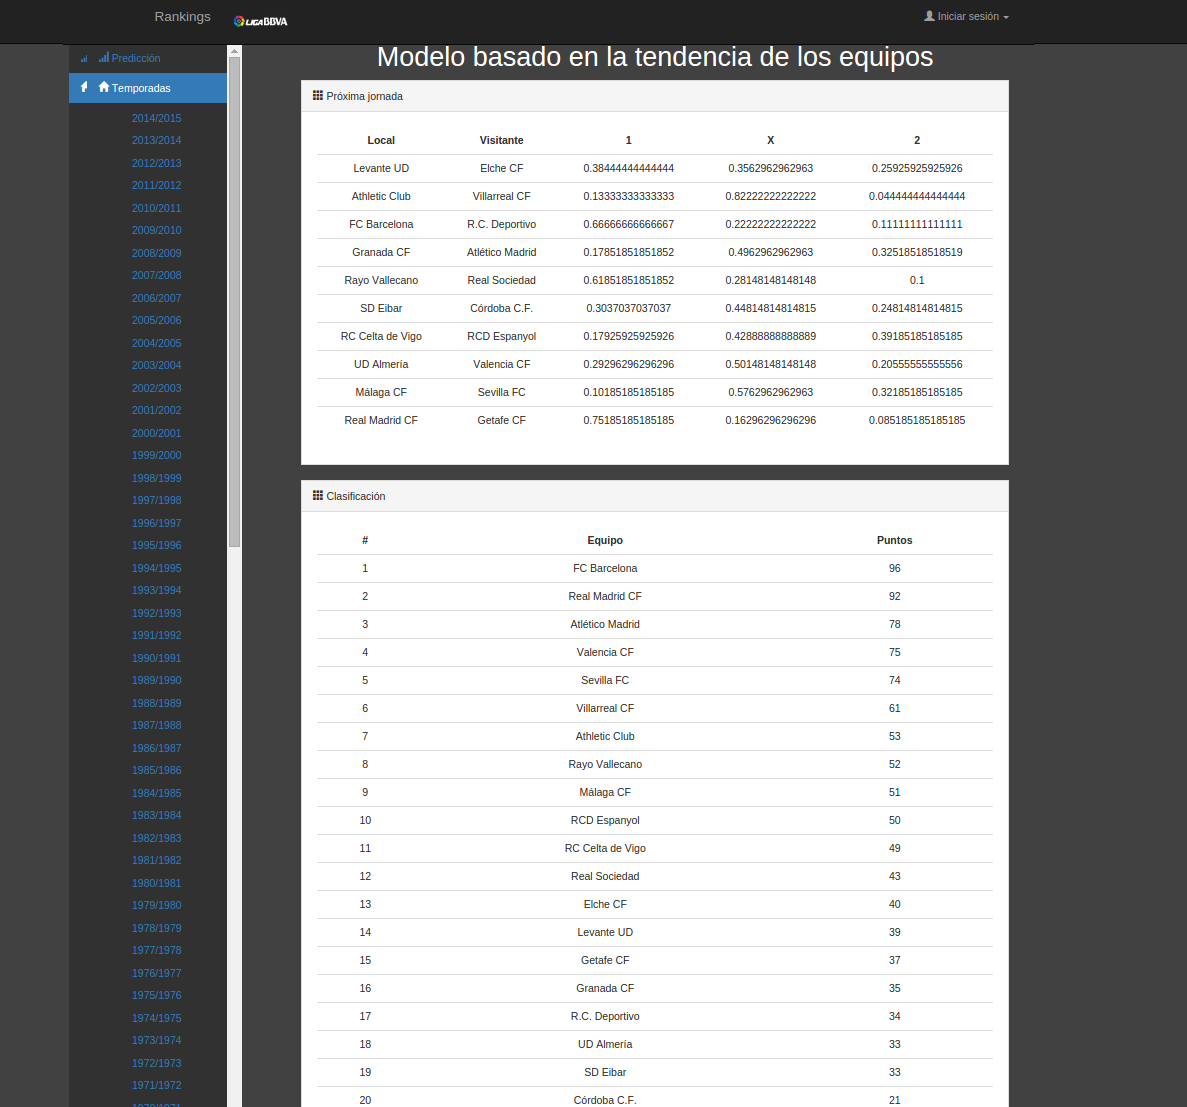
\includegraphics[scale=0.55]{images/pant_pred2.png}
	\caption{Vista del modulo de predicción(II).} \label{fig:pmod2}
\end{figure}
\begin{figure}[H]
	\centering
	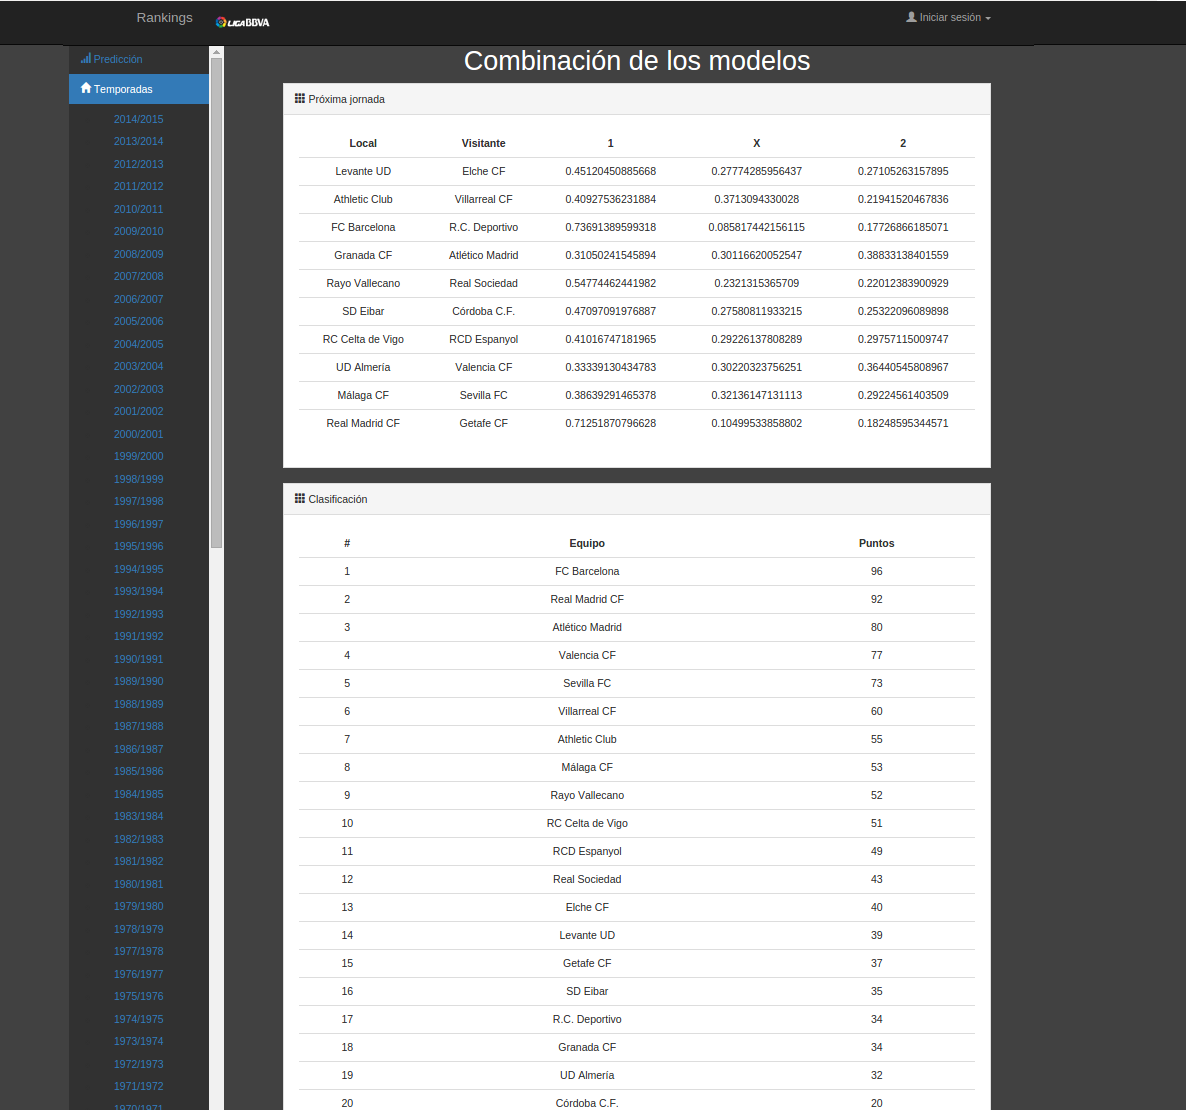
\includegraphics[scale=0.55]{images/pant_pred3.png}
	\caption{Vista del modulo de predicción(III).} \label{fig:pmod3}
\end{figure}	
	
	\appendix
	\chapter{Grafos}

A lo largo de la memoria mencionamos varias veces la palabra grafo. En este anexo introduciremos todos los conceptos relacionados con grafos y algunos ejemplos de los tipos de grafos más conocidos. El primero en hablar de grafos fue Euler en el año 1736 cuando resolvió el problema matemático de los siete puentes de Königsberg (la formulación y solución al problema se puede encontrar en \cite{refpuentes}) que dio origen a la teoría de grafos.\\

Pueden existir variantes de algunas de las definiciones que usaremos a continuación, la mayoría de las usadas han sido traducidas de \cite{librografos}.

\section{Conceptos básicos}

\begin{defi} 
	Un grafo (o grafo no dirigido) $G$ es un par ordenado $G=(V,E)$, donde:
	\begin{itemize}
		\item $V$ es un conjunto de vértices o nodos, y
		\item $E$ es un conjunto de aristas o arcos, que relacionan estos nodos.
	\end{itemize}
\end{defi}

Una arista que une dos nodos $v_{1},v_{2} \in V$ se denota como $v_{1}v_{2}$ o $v_{2}v_{1} \in E$. Cuando el nodo origen y el destino de una arista son el mismo estaremos hablando de bucles. Decimos que dos aristas son paralelas cuando ambas aristas relacionan el mismo par de vértices. Dos aristas son adyacentes si tienen un vértice en común, y dos vértices son adyacentes si existe una arista que los une.

\begin{defi} 
	El orden de un grafo $G$ es el número de vértices de $G$, es decir, $|V|$.
\end{defi}

Nos interesará estudiar los grafos finitos, cuando $|G|< \infty$, ya que muchos de los resultados sobre grafos no se pueden aplicar a grafos infinitos.

\begin{defi} 
	El grado de un nodo $v \in V$ se define como el número de aristas que lo tienen como extremo.
\end{defi}

\newpage

\begin{ejem} 
	En la figura \ref{fig:graph} se muestra un grafo donde $ V = \{1,2,3\} \text{  y  } E = \{12,23\} $.
\end{ejem}

\begin{figure}[H]
	\centering
	\begin{tikzpicture}[shorten >=1pt, auto, node distance=3cm, ultra thick]
	\tikzstyle{node_style} = [circle,draw=black,fill=black,font=\sffamily\Large\bfseries,text=white]
	\tikzstyle{edge_style} = [draw=black, line width=2, ultra thick]
	\node[node_style] (v1) at (0,2) {1};
	\node[node_style] (v2) at (-3,-2) {2};
	\node[node_style] (v3) at (3,-2) {3};
	\draw[edge_style] (v1) edge (v2);
	\draw[edge_style] (v2) edge (v3);
	\end{tikzpicture}
	\caption{Ejemplo de grafo.}
	\label{fig:graph}
\end{figure}

El orden del grafo es 3. \\
El grado de cada uno de los nodos es $$g(1)=g(3)=1$$  $$g(2)=2.$$\\
\qed

\begin{defi} 
	El grafo complementario de $G$ se denota $\bar{G}$ y tiene el mismo conjunto de vértices que $G$, pero su conjunto de aristas son todas aquellas que unen los vértices que no están unidos en $G$.
\end{defi}

\begin{ejem} 
	En la figura \ref{fig:graphcomplementario} se muestra el grafo complementario del de la figura \ref{fig:graph}.
\end{ejem}

\begin{figure}[H]
	\centering
	\begin{tikzpicture}[shorten >=1pt, auto, node distance=3cm, ultra thick]
	\tikzstyle{node_style} = [circle,draw=black,fill=black,font=\sffamily\Large\bfseries,text=white]
	\tikzstyle{edge_style} = [draw=black, line width=2, ultra thick]
	\node[node_style] (v1) at (0,2) {1};
	\node[node_style] (v2) at (-3,-2) {2};
	\node[node_style] (v3) at (3,-2) {3};
	\draw[edge_style] (v1) edge (v3);
	\end{tikzpicture}
	\caption{Ejemplo de grafo complementario.}
	\label{fig:graphcomplementario}
\end{figure}

\qed

\begin{defi} 
	Dado un grafo $G=(V,E)$. Un camino de $v_{0}$ a $v_{n}$ es una sucesión de aristas $e_{1},e_{2},\dots,e_{n}$ de la forma $e_{1}=v_{0}v_{1}$, $e_{2}=v_{1}v_{2}$, $\dots$, $e_{n}=v_{n-1}v_{n}$, donde $v_{0}$ es el inicio del camino, $v_{n}$ es el fin del camino y la longitud del camino viene dada por el número de aristas de éste.
\end{defi}

\section{Tipos de grafos}

Existen multitud de tipos de grafos diferentes. Ya hemos mencionado algunos como los grafos no dirigidos, los grafos finitos y los infinitos. Vamos a presentar algunos tipos más:
\begin{itemize}
	\item Grafo nulo: es un grafo cuyos vértices no tienen ninguna arista que los una.
	
	\begin{figure}[H]
		\centering
		\begin{tikzpicture}[shorten >=1pt, auto, node distance=3cm, ultra thick]
		\tikzstyle{node_style} = [circle,draw=black,fill=black,font=\sffamily\Large\bfseries,text=white]
		\tikzstyle{edge_style} = [draw=black, line width=2, ultra thick]
		\node[node_style] (v1) at (0,2) {1};
		\node[node_style] (v2) at (-3,-2) {2};
		\node[node_style] (v3) at (3,-2) {3};
		\end{tikzpicture}
		\caption{Ejemplo de grafo nulo.}
		\label{fig:grafonulo}
	\end{figure}
	
	\item Grafo simple: es un grafo que no posee bucles ni aristas paralelas. Los ejemplos que hemos visto hasta ahora son todos grafos simples.
	\item Multigrafo: $G$ es un multigrafo si y solo si no es simple, es decir, tiene bucles y/o aristas paralelas.
	
	\begin{figure}[H] 
		\centering
		\tikzset{me/.style={to path={
			\pgfextra{
				\pgfmathsetmacro{\startf}{-(#1-1)/2}  
				\pgfmathsetmacro{\endf}{-\startf} 
				\pgfmathsetmacro{\stepf}{\startf+1}}
			\ifnum 1=#1 -- (\tikztotarget)  \else
			\foreach \i in {\startf,\stepf,...,\endf}
			{
				(\tikztostart) parabola[bend pos=0.5] bend +(0,0.4*\i)  (\tikztotarget)
			}
			\fi   
			\tikztonodes
		}}}  			
		
		\begin{tikzpicture}[shorten >=1pt, auto, node distance=3cm, ultra thick,every loop/.style=]
			\tikzstyle{node_style} = [circle,draw=black,fill=black,font=\sffamily\Large\bfseries,text=white]
			\tikzstyle{edge_style} = [draw=black, line width=2, ultra thick]
			\node[node_style] (v1) at (0,2) {1};
			\node[node_style] (v2) at (-3,-2) {2};
			\node[node_style] (v3) at (3,-2) {3};
			\draw[edge_style] (v1) edge (v2);
			\draw[thick] (v2) edge[me=5] (v3); 
			\path[thick] (v1) edge [loop above] ();
			\path[thick] (v2) edge [loop left] ();
			\path[thick] (v3) edge [loop right] ();
		\end{tikzpicture}
		\caption{Ejemplo multigrafo.}
	\end{figure}
	
	\newpage
	
	\item Grafo completo: es un grafo simple que cumple que para cada par de vértices del grafo existe una arista que los une, es decir, contiene todas las aristas posibles.
	
	\begin{figure}[H]
		\centering
		\begin{tikzpicture}[shorten >=1pt, auto, node distance=3cm, ultra thick]
		\tikzstyle{node_style} = [circle,draw=black,fill=black,font=\sffamily\Large\bfseries,text=white]
		\tikzstyle{edge_style} = [draw=black, line width=2, ultra thick]
		\node[node_style] (v1) at (0,2) {1};
		\node[node_style] (v2) at (-3,-2) {2};
		\node[node_style] (v3) at (3,-2) {3};
		\draw[edge_style] (v1) edge (v2);
		\draw[edge_style] (v1) edge (v3);
		\draw[edge_style] (v2) edge (v3);
		\end{tikzpicture}
		\caption{Ejemplo de grafo completo.}
		\label{fig:grafocompleto}
	\end{figure}
	Nótese que cuando tenemos el mismo conjunto de vértices $V$, el grafo nulo y el grafo completo son complementarios. Por ejemplo, el grafo de la figura \ref{fig:grafonulo} y el de la figura \ref{fig:grafocompleto} son complementarios.

	\item Grafo regular: es un grafo en el que todos los nodos tienen el mismo grado. Por ejemplo el grafo de la figura \ref{fig:grafocompleto} es un grafo regular.

	\item Grafo conexo: es un grafo que cumple que para cada par de nodos existe al menos un camino que los une. La mayoría de grafos vistos hasta ahora son conexos. El grafo de la figura \ref{fig:graphcomplementario} es un grafo no conexo ya que el vértice 2 no tiene ningún camino que lo una a 1 y 3.
	
	\item  Árbol: son grafos que conectan todos los vértices utilizando el menor número posible de aristas. Tienen $n$ nodos y $n-1$ aristas.
	
	\begin{figure}[H]
		\centering
		\begin{tikzpicture}[shorten >=1pt, auto, node distance=3cm, ultra thick]
		\tikzstyle{node_style} = [circle,draw=black,fill=black,font=\sffamily\Large\bfseries,text=white]
		\tikzstyle{edge_style} = [draw=black, line width=2, ultra thick]
		\node[node_style] (v1) at (0,2) {1};
		\node[node_style] (v2) at (-3,-2) {2};
		\node[node_style] (v3) at (3,-2) {3};
		\draw[edge_style] (v1) edge (v2);
		\draw[edge_style] (v1) edge (v3);
		\end{tikzpicture}
		\caption{Ejemplo de árbol.}
	\end{figure}

	\newpage

	\item Grafo dirigido: es un tipo de grafo en el cual las aristas tienen una dirección definida, tienen un nodo de inicio y uno de fin. En un grafo dirigido las aristas $v_{1}v_{2}$ y $v_{2}v_{1}$ son distintas.
	
	\begin{figure}[H]
		\centering
		\begin{tikzpicture}[shorten >=1pt, auto, node distance=3cm, ultra thick]
		\tikzstyle{node_style} = [circle,draw=black,fill=black,font=\sffamily\Large\bfseries,text=white]
		\tikzstyle{edge_style} = [draw=black, line width=2, ultra thick,->]
		\node[node_style] (v1) at (0,2) {1};
		\node[node_style] (v2) at (-3,-2) {2};
		\node[node_style] (v3) at (3,-2) {3};
		\draw[edge_style] (v1) edge (v2);
		\draw[edge_style] (v1) edge (v3);
		\draw[edge_style] (v2) edge (v3);
		\end{tikzpicture}
		\caption{Ejemplo de grafo dirigido.}
	\end{figure}	
	
	\item Grafo ponderado: es un grafo que asocia un número real (peso o ponderación) a cada arista. Estos grafos se suelen aplicar a problemas de optimización como por ejemplo para hallar el camino más corto.
	
		\begin{figure}[H]
			\centering
			\begin{tikzpicture}[shorten >=1pt, auto, node distance=3cm, ultra thick]
			\tikzstyle{node_style} = [circle,draw=black,fill=black,font=\sffamily\Large\bfseries,text=white]
			\tikzstyle{edge_style} = [draw=black, line width=2, ultra thick,->]
			\node[node_style] (v1) at (0,2) {1};
			\node[node_style] (v2) at (-3,-2) {2};
			\node[node_style] (v3) at (3,-2) {3};
			\Edge[label=$45$](v1)(v2)
			\Edge[label=$50$](v1)(v3)
			\Edge[label=$20$](v2)(v3)
			\end{tikzpicture}
			\caption{Ejemplo de grafo ponderado.}
		\end{figure}

\end{itemize}

\newpage

\section{Representación de grafos}

Además de la geométrica, existen diferentes formas de representar un grafo, vamos a ver algunas formas alternativas que nos pueden ser útiles para almacenarlos en un computador. 

\begin{figure}[H]
	\centering
	\begin{tikzpicture}[shorten >=1pt, auto, node distance=3cm, ultra thick]
	\tikzstyle{node_style} = [circle,draw=black,fill=black,font=\sffamily\Large\bfseries,text=white]
	\tikzstyle{edge_style} = [draw=black, line width=2, ultra thick]
	\node[node_style] (A) at (-2,2) {A};
	\node[node_style] (B) at (2,2) {B};
	\node[node_style] (C) at (-2,-2) {C};
	\node[node_style] (D) at (2,-2) {D};
	\draw[edge_style] (A) edge (B);
	\draw[edge_style] (B) edge (C);
	\draw[edge_style] (C) edge (D);	
	\end{tikzpicture}
	\caption{Ejemplo de grafo.}
	\label{fig:graphrep}
\end{figure}

\begin{itemize}
	\item Lista de adyacencia: cada vértice tiene una lista asociada con los vértices adyacentes a él. En grafos no dirigidos se produce redundancia.\\
	La lista de adyacencia asociada al grafo \ref{fig:graphrep} es $\{\{B\},\{A,C\},\{B,D\},\{C\}\}$.
	\item Lista de grados: es una secuencia de números, que se corresponden con los grados de los vértices del grafo.\\
	La lista de de grados asociada al grafo \ref{fig:graphrep} es $\{2,2,1,1\}$.
	
	\item Matriz de adyacencia: el grafo está representado por una matriz cuadrada $M_{nxn}$, donde $n$ es el número de vértices del grafo. Si hay una arista entre un vértice $v_{i}$ y un vértice $v_{j}$, entonces el elemento $m_{i,j}$ toma el valor 1, si no toma el valor 0. En el caso de grafos simples la diagonal principal estará formada por ceros.\\
	La matriz de adyacencia asociada al grafo \ref{fig:graphrep} es
	\renewcommand{\kbldelim}{(}
	\renewcommand{\kbrdelim}{)}
	\[\kbordermatrix{
		& A & B & C & D\\
		A & 0 & 1 & 0 & 0\\
		B & 1 & 0 & 1 & 0\\
		C & 0 & 1 & 0 & 1\\
		D & 0 & 0 & 1 & 0
	}.
	\]
	
	\item Matriz de incidencia: el grafo está representado por una matriz $M_{mxn}$, donde $m$ es el número de vértices y $n$ el número de aristas del grafo. Si el vértice $v_{i}$ y la arista $e_{j}$ están conectados, entonces el elemento $m_{i,j}$ toma el valor 1, si no toma el valor 0.\\
	La matriz de incidencia asociada al grafo \ref{fig:graphrep} es
	\renewcommand{\kbldelim}{(}
	\renewcommand{\kbrdelim}{)}
	\[\kbordermatrix{
		& ab & bc & cd\\
		A & 1 & 0 & 0\\
		B & 1 & 1 & 0\\
		C & 0 & 1 & 1\\
		D & 0 & 0 & 1
	}.
	\]
	
\end{itemize}


	
\newpage

\section{Teoría de grafos}

Gracias a la teoría de grafos se pueden resolver problemas en áreas muy distintas.  Algunos de sus muchos usos son: modelización de trayectos en redes de transporte en las que nos interesa obtener caminos óptimos aplicando diversos algoritmos como puede ser el de Floyd, en administración de proyectos se utilizan técnicas como la de revisión y evaluación de programas (PERT) en las que se modela utilizando grafos y optimizando los tiempos, en redes sociales para estudiar la influencia de determinadas personas dentro de círculos de gente, en biología y ecología se aplica a redes tróficas para estudiar como afectaría la extinción de algunas especies a todo el hábitat, etc.\\

\begin{figure}[H]
	\centering
	\subfloat[Prb. Puentes de Königsberg]{
		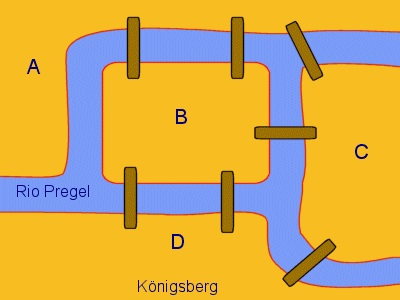
\includegraphics[width=0.3\textwidth]{images/aplicaciones1.jpg}}
	\subfloat[Plano de metro]{
		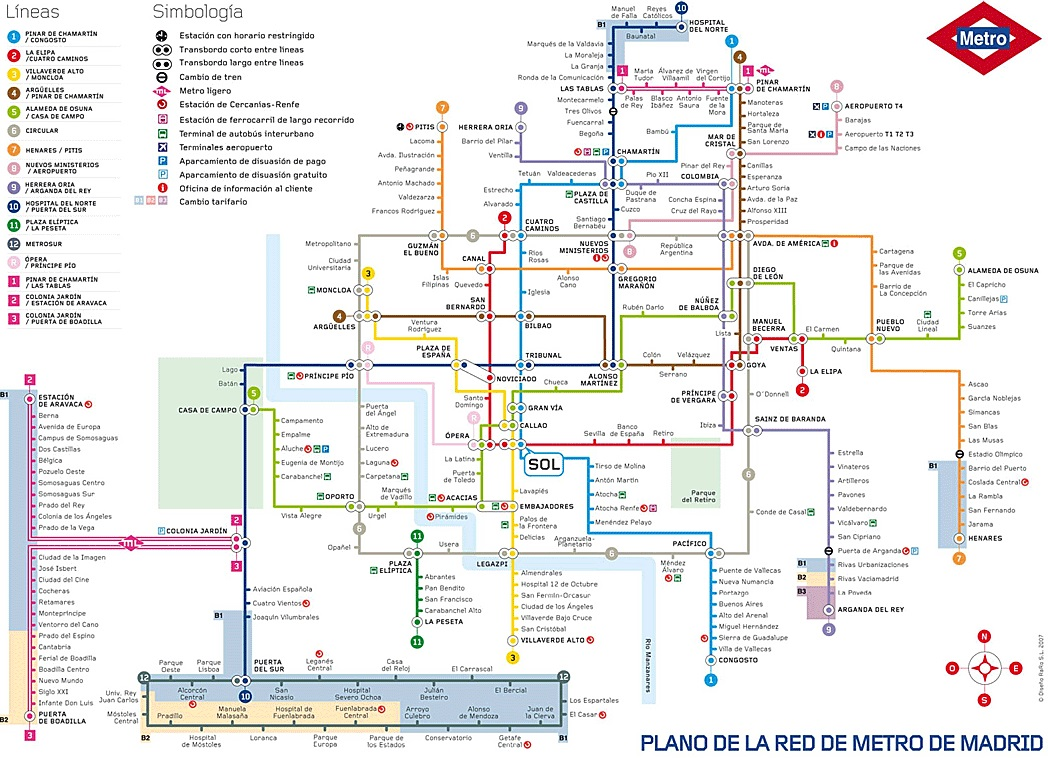
\includegraphics[width=0.3\textwidth]{images/aplicaciones2.jpg}}
	\subfloat[Moléculas]{
		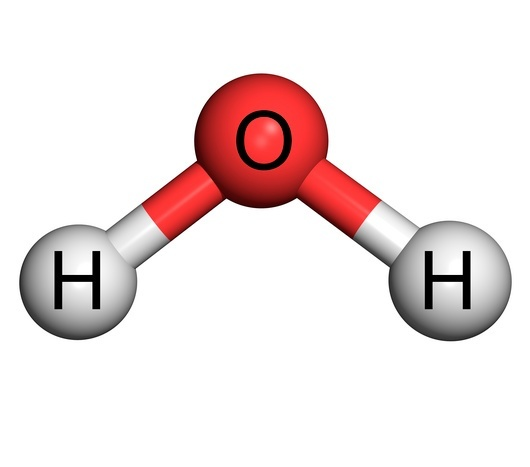
\includegraphics[width=0.3\textwidth]{images/aplicaciones3.jpg}}\\
	\subfloat[Red de computadoras]{
		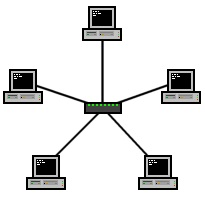
\includegraphics[width=0.3\textwidth]{images/aplicaciones4.jpg}}
	\subfloat[Cadena trófica]{
		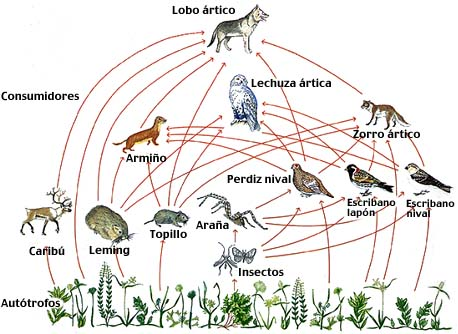
\includegraphics[width=0.3\textwidth]{images/aplicaciones5.jpg}}
	\subfloat[Redes sociales]{
		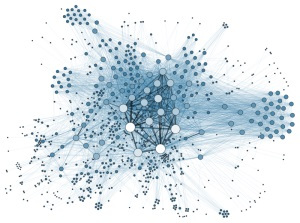
\includegraphics[width=0.3\textwidth]{images/aplicaciones6.jpg}}\\
	\subfloat[Teo. seis grados de separación]{
		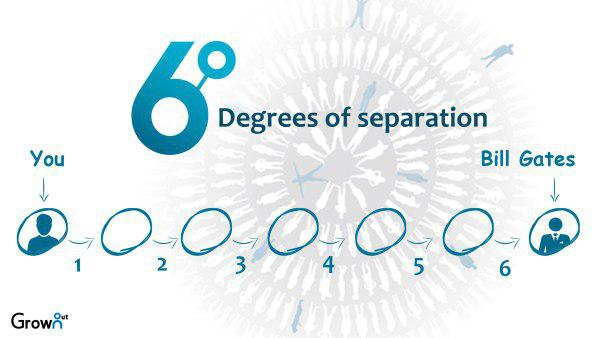
\includegraphics[width=0.3\textwidth]{images/aplicaciones7.jpg}}
	\subfloat[Prb. Coloreado de mapas]{
		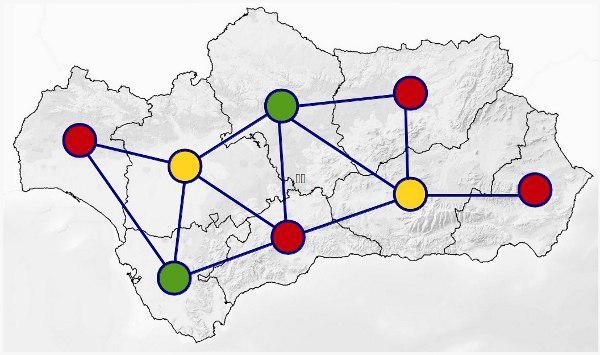
\includegraphics[width=0.3\textwidth]{images/aplicaciones8.jpg}}
	\subfloat[Diagrama de PERT]{
		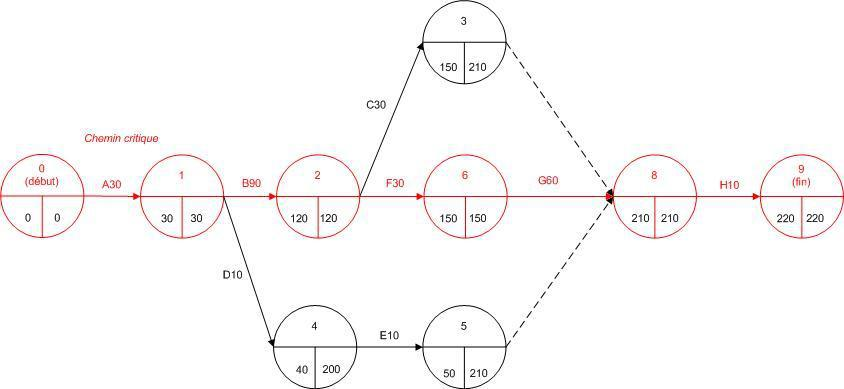
\includegraphics[width=0.3\textwidth]{images/aplicaciones9.jpg}}	
	\caption{Múltiples aplicaciones de teoría de grafos.}
\end{figure}

	\chapter{Resultados de la Liga Endesa 2014/2015}
Este anexo consta de varias tablas con los rankings y resultados de la temporada 2014/2015 de la Liga Endesa \cite{acbresults} que hemos usado en los ejemplos del Capítulo 2.\\

\section*{Equipos participantes}

\begin{figure}[H]
	\centering
	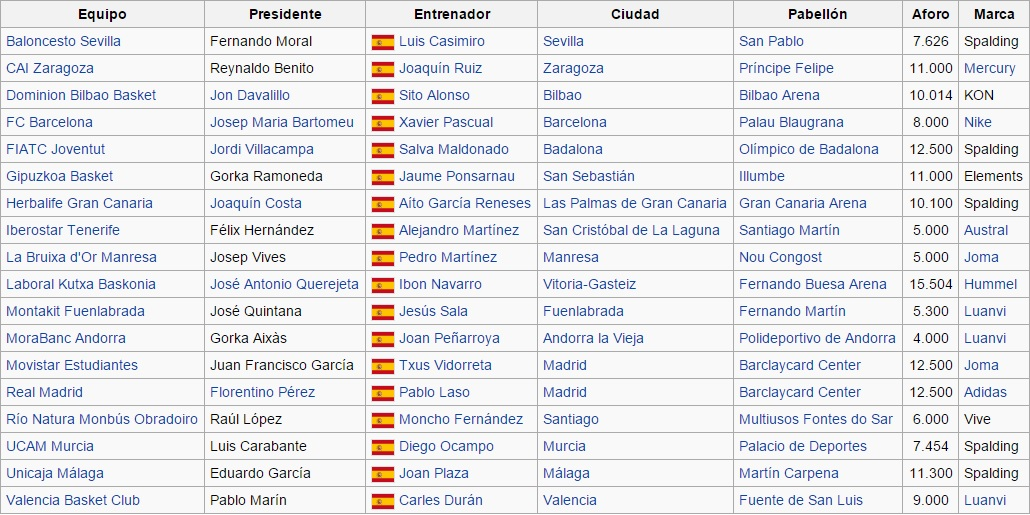
\includegraphics[scale=0.6]{images/equipos.jpg}
	\caption{Tabla de equipos.} 
\end{figure}

\section*{Ranking de la liga regular}

\begin{figure}[H]
	\centering
	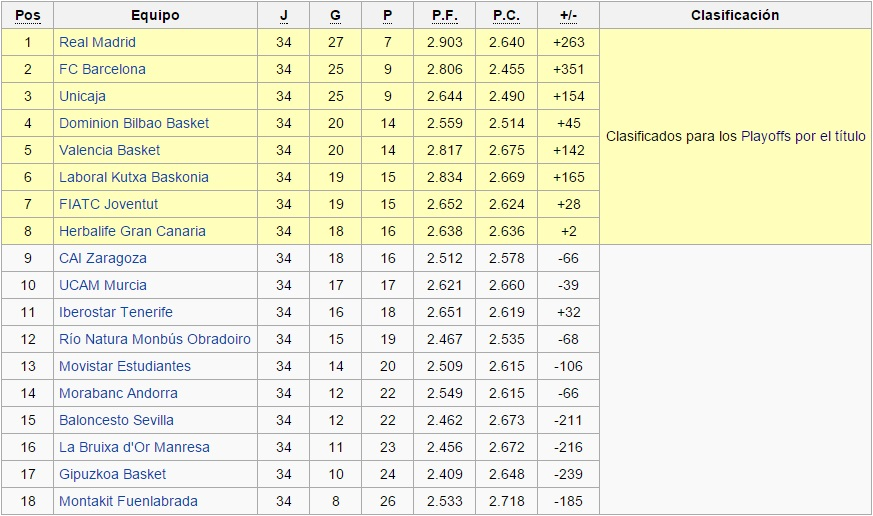
\includegraphics[scale=0.7]{images/regular.jpg}
	\caption{Ranking al finalizar la liga regular.} 
\end{figure}

\section*{Resultados de la liga regular}

\begin{figure}[H]
	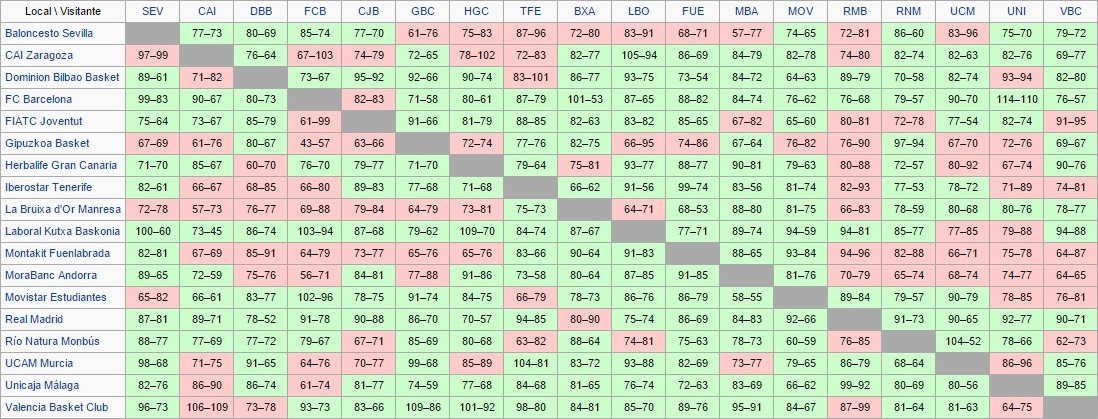
\includegraphics[scale=0.6]{images/resultados.jpg}
	\caption{Tabla de resultados de la liga regular.} 
\end{figure}

\section*{Evolución de la clasificación}

\begin{figure}[H]
	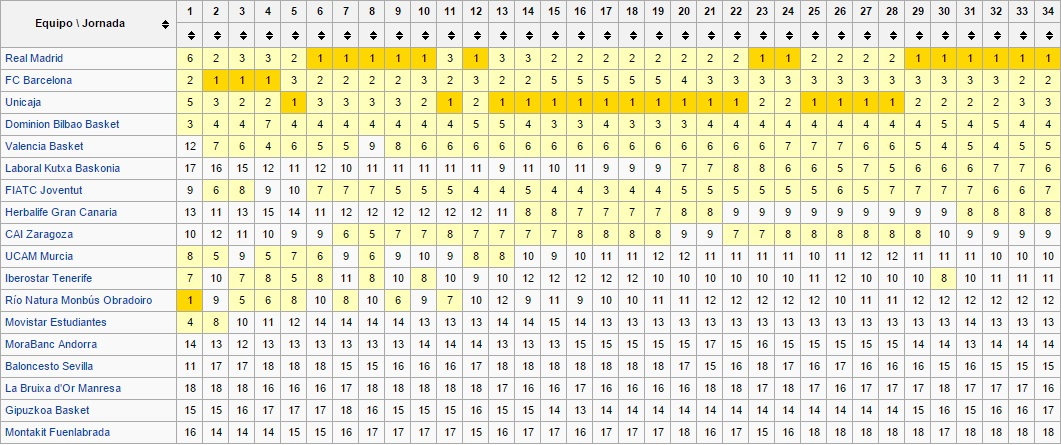
\includegraphics[scale=0.6]{images/evolucion.jpg}
	\caption{Tabla con la evolución de la clasificación.} 
\end{figure}

\section*{Playoffs}

\begin{figure}[H]
	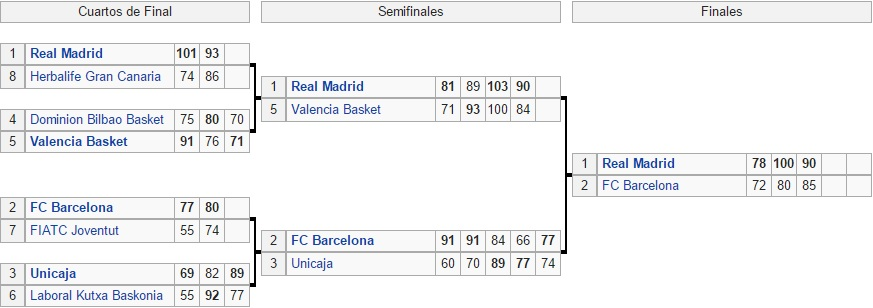
\includegraphics[scale=0.7]{images/playoffs.jpg}
	\caption{Tabla de resultados de los playoffs.} 
\end{figure}

\section*{Clasificación final}

\begin{figure}[H]
	\centering
	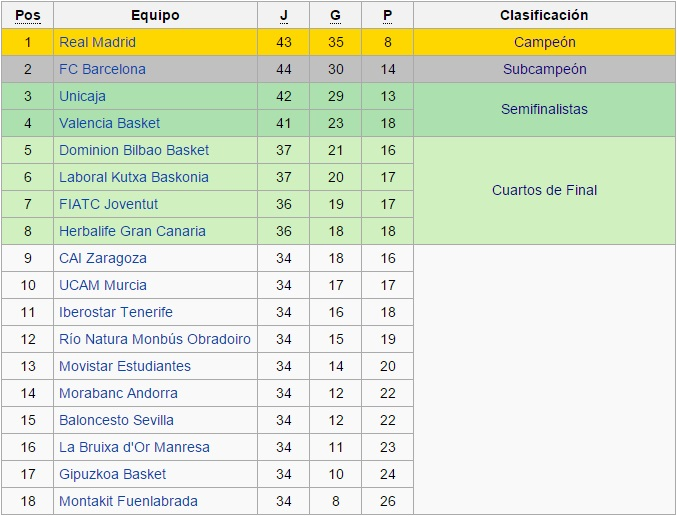
\includegraphics[scale=0.8]{images/final.jpg}
	\caption{Ranking final.} 
\end{figure}
	\definecolor{mygreen}{RGB}{28,172,0} % color values Red, Green, Blue
\definecolor{mylilas}{RGB}{170,55,241}

\lstset{language=Matlab,%
	%basicstyle=\color{red},
	breaklines=true,%
	morekeywords={matlab2tikz},
	keywordstyle=\color{blue},%
	morekeywords=[2]{1}, keywordstyle=[2]{\color{black}},
	identifierstyle=\color{black},%
	stringstyle=\color{mylilas},
	commentstyle=\color{mygreen},%
	showstringspaces=false,%without this there will be a symbol in the places where there is a space
	%numbers=left,%
	%numberstyle={\tiny \color{black}},% size of the numbers
	%numbersep=9pt, % this defines how far the numbers are from the text    
}

\chapter{Código MATLAB}

\section{Métodos para crear rankings}

\subsection*{Método de Massey}
\fbox{\parbox[b]{\linewidth}{
		\lstinputlisting{../matlabcode/massey.m}			
}}

\newpage

\subsection*{Método de Colley}

\fbox{\parbox[b]{\linewidth}{
		\lstinputlisting{../matlabcode/colley.m}			
}}


\subsection*{Método de Keener}

\fbox{\parbox[b]{\linewidth}{
		\lstinputlisting{../matlabcode/keener.m}			
}}

\subsection*{Método de ataque-defensa}

\fbox{\parbox[b]{\linewidth}{
		\lstinputlisting{../matlabcode/ataque.m}			
}}
\ \\

\fbox{\parbox[b]{\linewidth}{
		\lstinputlisting{../matlabcode/defensa.m}			
}}

\newpage

\section{Parámetros de entrada para los ejemplos}

\subsection*{Parámetros Massey}

\fbox{\parbox[b]{\linewidth}{
		\lstinputlisting{../matlabcode/entradas_massey.txt}			
}}
	
\newpage	
	
\subsection*{Parámetros Colley}

\fbox{\parbox[b]{\linewidth}{
		\lstinputlisting{../matlabcode/entradas_colley.txt}			
}}

\newpage

\subsection*{Parámetros Keener}

\fbox{\parbox[b]{\linewidth}{
		\lstinputlisting{../matlabcode/entradas_keener.txt}			
}}

\newpage

\subsection*{Parámetros ataque-defensa}

\fbox{\parbox[b]{\linewidth}{
		\lstinputlisting{../matlabcode/entradas_od.txt}			
}}
	\definecolor{pblue}{rgb}{0.13,0.13,1}
\definecolor{pgreen}{rgb}{0,0.5,0}
\definecolor{pred}{rgb}{0.9,0,0}
\definecolor{pgrey}{rgb}{0.46,0.45,0.48}

\lstset{language=Java,
	showspaces=false,
	showtabs=false,
	breaklines=true,
	showstringspaces=false,
	breakatwhitespace=true,
	commentstyle=\color{pgreen},
	keywordstyle=\color{pblue},
	stringstyle=\color{pred},
	basicstyle=\ttfamily,
	moredelim=[il][\textcolor{pgrey}]{$$},
	moredelim=[is][\textcolor{pgrey}]{\%\%}{\%\%}
}

\chapter{Código Java}
En este anexo se incluye el código en Java (por su mayor simplicidad para la programación requerida) de los ejemplos realizados en la sección 2.4.
\section{Métodos de comparación de rankings}

\subsection*{Tau de Kendall}
\fbox{\parbox[b]{\linewidth}{
		\lstinputlisting{../javacode/TauKendall.java}			
}}

\subsection*{Rho de Spearman}
\fbox{\parbox[b]{\linewidth}{
		\lstinputlisting{../javacode/RhoSpearman.java}			
}}

\subsection*{Función devolver}
\fbox{\parbox[b]{\linewidth}{
		\lstinputlisting{../javacode/Devolver.java}			
}}

\section{Rankings usados en los ejemplos}
\fbox{\parbox[b]{\linewidth}{
		\lstinputlisting{../javacode/Ejemplos.java}			
}}	
	
	
	\backmatter
	\begin{thebibliography}{X}
		\bibitem{libro_rankings} \textsc{A. N. Langville, C. D. Meyer},
		\textit{Who's \#1? The science of rating and ranking}, 
		Princeton University Press, Princeton, 2012.
		\bibitem{laplace}
		Artículo sobre la regla de sucesión de Laplace (Castellano). \url{https://es.wikipedia.org/wiki/Regla_de_sucesion}			
		\bibitem{perron} \textsc{C. D. Meyer},
		\textit{Matrix analysis and applied linear algebra}, 
		SIAM, Philadelphia, 2000. 
		\bibitem{power_method}
		Artículo sobre el método de las potencias en Wikipedia (Inglés). \url{https://en.wikipedia.org/wiki/Power_iteration}
		\bibitem{refborda} \textsc{E. B. Burger, M. Starbird},
		\textit{The Heart of Mathematics. An invitation to effective thinking}, 
		Third Edition, John Wiley \& Sons, 2010.		
		\bibitem{refbilp} \textsc{K. E. Pedings, A. N. Langville, Y. Yamamoto}, ``A Minimum Violations Ranking Method'',
		\textit{Optimization and Engineering}, Volume 13(2) (2012), 349-370.
		\bibitem{refcomp} \textsc{R. Criado, E. García, F. Pedroche, M. Romance}, ``On graphs associated to sets of rankings'',
		\textit{Journal of Computational and Applied Mathematics}, Volume 291 (2016), 497–508.
		\bibitem{refpred1} \textsc{M. Spann, B. Skiera}, ``Sports forecasting: A comparison of the forecast accuracy of prediction markets, betting odds and tipsters'', \textit{Journal of Forecasting}, Volume 28 (2009), 55-72.
		\bibitem{refpred2} \textsc{T. Cheng, D. Cui, Z. Fan, J. Zhou, S. Lu}, ``A new model to forecast the results of matches based on hybrid neural networks in the soccer rating system'', \textit{Computational Intelligence and Multimedia Applications} (2003), 308-313. 
		\bibitem{refpred3} \textsc{G. Hiranandani, J. Shitole, N. Kundu, N. Maurya, R. Grover},
		"Forecasting Indian Premier League Results Using Time Series Analysis", 
		2013. 	
		\bibitem{tfgjavi} \textsc{Javier Jiménez del Peso},
		\textit{Diseño e implementación de modelos de predicción para la Liga BBVA}, 
		Trabajo Fin de Grado de Ingeniería de Informática, 2016.			
		\bibitem{refpuentes}
		Artículo sobre el problema de los puentes de Königsberg en Wikipedia (Castellano). \url{https://es.wikipedia.org/wiki/Problema_de_los_puentes_de_Konigsberg}
		\bibitem{librografos} \textsc{W. Kocay, D. L. Kreher},
		\textit{Graphs, algorithms, and optimization}, 
		Chapman and Hall/CRC, 2004.
		\bibitem{acbresults}
		Artículo sobre la Liga ACB 2014-15 en Wikipedia (Castellano). \url{https://es.wikipedia.org/wiki/Liga_ACB_2014-15}
	\end{thebibliography}

	
	
\end{document}